\part{Conceptes elementals de programació}


\chapter{Repetir}
\label{cap7}

\includegraphics[scale=0.135]{Imatges/figura7-0.jpg}

Ara per ara, segur que penseu que la feina del programador de robots és força tediosa. Probablement teniu bones idees per fer dibuixos interessants, però no us veieu amb cor  d'escriure els \emph{scripts} per fer-los realitat, ja que sembla que el nombre de línies que heu d'escriure creix a mida que la complexitat del dibuix augmenta. En aquest capítol aprendreu a utilitzar \emph{repeticions} (també conegudes com \emph{bucles}) per reduir el nombre d'expressions que cal donar als robots. Les repeticions us permeten \emph{repetir una seqüència d'expressions}. Amb un bucle, l'\emph{script} per dibuixar un hexàgon o un octàgon no és pas més gran que l'\emph{script} per dibuixar un quadrat.

\section{Ha nascut una estrella}
\index{dibuixar!estrella|(}
\index{estrella!dibuixar|(}
Ens agradaria que un robot dibuixés una estrella, semblant a la que teniu dibuixada al començament d'aquest capítol. Ho farem de la seguent manera: començant des del que serà el centre de l'estrella, el robot dibuixa una línia, retorna al centre, gira un determinat angle, dibuixa una altra línia, i així fins que l'estrella s'acabi. L'\emph{Script}~\ref{scr7-1} crea un robot que dibuixa una línia de 70 píxels de llarg i retorna al lloc d'on ha sortit. Fixeu-vos que  després de tornar al lloc de partida, el robot fa mitja volta, i així apunta en la direcció original.
\begin{script}  Dibuixar una línia i tornar al lloc de partida.
\textsf{\upshape
\\
\\$|$ pica $|$\\
pica := Bot nou.\\
pica ves: 70.\\
pica giraEsquerra: 180.\\
pica ves: 70.\\
pica giraEsquerra: 180.\\
}
\label{scr7-1}
\end{script}

Per dibuixar una estrella, hem de repetir part de l'\emph{script}~\ref{scr7-1} i després ordenar al robot que giri un angle determinat. Si volem dibuixar una estrella de sis puntes, l'angle ha de ser de 60 graus, ja que girant 60 graus cada vegada resultarà en $360/60 = 6$ branques. L'\emph{Script}~\ref{scr7-2} ens mostra com hem de fer això per obtenir una estrella amb 6 branques sense utilitzar repeticions. \index{linies@línies!dibuixar per a una estrella}

\begin{script}  Una estrella de sis puntes sense utilitzar repeticions.
\textsf{\upshape
\\
\\$|$ pica $|$\\
pica := Bot nou.\\
pica ves: 70.\\
pica giraEsquerra: 180.\\
pica ves: 70.\\
pica giraEsquerra: 180.\\
pica giraEsquerra: 60.\\
{\itshape
pica ves: 70.\\
pica giraEsquerra: 180.\\
pica ves: 70.\\
pica giraEsquerra: 180.\\
pica giraEsquerra: 60.\\
}
pica ves: 70.\\
pica giraEsquerra: 180.\\
pica ves: 70.\\
pica giraEsquerra: 180.\\
pica giraEsquerra: 60.\\
{\itshape
pica ves: 70.\\
pica giraEsquerra: 180.\\
pica ves: 70.\\
pica giraEsquerra: 180.\\
pica giraEsquerra: 60.\\
}
pica ves: 70.\\
pica giraEsquerra: 180.\\
pica ves: 70.\\
pica giraEsquerra: 180.\\
pica giraEsquerra: 60.\\
{\itshape
pica ves: 70.\\
pica giraEsquerra: 180.\\
pica ves: 70.\\
pica giraEsquerra: 180.\\
pica giraEsquerra: 60.\\
}}
\label{scr7-2}
\end{script}

Com podeu veure, després ser creat, \textsf{pica} repeteix les mateixes cinc línies de codi sis vegades (ho hem mostrat alternant el tipus normal amb lletra itàlica). Sembla una pèrdua de temps haver d'escriure el mateix tros de codi una vegada i una altra. Imagineu la mida del vostre \emph{script} si volguéssiu una estrella amb 60 branques, com la que mostrem a l'Experiment 7-1. El que ens cal és una manera de repetir una seqüència d'expressions.

\subsection{Bucles al rescat}
\index{missatges!utilitzar bucles amb|(}
\index{vegadesRepetir: mètode!efecte de}
La solució del nostre problema és utilitzar un \emph{bucle}. Hi ha diferents tipus de bucles, i el que introduirem ara us permet repetir una seqüència donada de missatges un nombre donat de vegades. El mètode\footnote{\emph{Nota del Traductor:} \textsf{timesRepeat:} en la versió original de Smalltalk} \textsf{vegadesRepetir:} repeteix una seqüència d'expressions un cert nombre de vegades, com veieu a l'\emph{Script}~\ref{scr7-3}. Aquest \emph{script} defineix la mateixa estrella que l'\emph{Script}~\ref{scr7-2}, però amb molt menys codi. Fixeu-vos que les expressions que s'han de repetir estan col·locades entre claudàtors.\index{bucles!repetir seq{\"u}ències de missatges en|(} \index{n vegadesRepetir: [], efecte de}
\begin{script}  Dibuixar una estrella de sis puntes utilitzant un bucle.
\textsf{\upshape
\begin{tabbing}
\hspace{5mm} \= \kill
$|$ pica $|$\\
pica := Bot nou.\\
6 vegadesRepetir:\\
\> {\bfseries [  pica ves: 70.}\\
\> {\bfseries pica giraEsquerra: 180.}\\
\> {\bfseries pica ves: 70.}\\
\> {\bfseries pica giraEsquerra: 180.}\\
\> {\bfseries pica giraEsquerra: 60.  ]}\\
\end{tabbing}
}
\label{scr7-3}
\end{script}

\noindent
\rule{\textwidth}{2pt}
\noindent
\textbf{Important!} \textsf{{\itshape n} vegadesRepetir: [ {\itshape seqüència d'expressions} ]} repeteix una seqüència d'expressions \textsf{{\itshape n}} vegades.\\
\noindent
\rule{\textwidth}{2pt}
\vspace{3mm}

El mètode \textsf{vegadesRepetir:} permet repetir una seqüència d'expressions, i a Smalltalk, aquesta seqüència d'expressions delimitada per claudàtors s'anomena \emph{bloc}. \index{Smalltalk!blocs (\emph{block})}\index{[] (claudàtors)!utilitzar en repeticions} \index{claudàtors ([])!utilitzar en repeticions}

El missatge \textsf{vegadesRepetir:} s'envia a un nombre enter, el nombre de vegades que la seqüència s'hauria de repetir. A l'\emph{Script}~\ref{scr7-3} el missatge \textsf{vegadesRepetir: [ \dots ]} és enviat a l'enter \textsf{6}. Res de nou aquí; ja vau veure un missatge enviat a un nombre enter quan vam parlar de la suma: el segon enter és enviat al primer, que retorna la suma dels dos.

Finalment, fixeu-vos que el nombre receptor del missatge \textsf{vegadesRepetir:} ha de ser un \emph{nombre enter} ja que en un bucle, igual que a la vida real, no està clar què vol dir executar una seqüència d'expressions, diguem, 0.2785 vegades.

L'argument de \textsf{vegadesRepetir:} és un bloc, és a dir, una seqüència d'expressions envoltada per un parell de claudàtors. Recordeu del capítol~\ref{cap2} que l'argument d'un missatge consisteix en la informació que l'objecte receptor necessita per executar el missatge. Per exemple, \textsf{[ pica ves: 70. pica giraEsquerra: 180. pica ves: 70. ]} és un bloc compost de tres expressions: \textsf{pica ves: 70}, \textsf{pica giraEsquerra: 180} i \textsf{pica ves: 70}. \index{vegadesRepetir: mètode!arguments de} \index{timesRepeat:|see{vegadesRepetir:}}

\noindent
\rule{\textwidth}{2pt}
\noindent
\textbf{Important!} L'argument de \textsf{vegadesRepetir:} és un \emph{bloc}, això és, una seqüència d'expressions entre claudàtors.\\
\noindent
\rule{\textwidth}{2pt}

\subsection{Repeticions en marxa}

Si compareu l'\emph{Script}~\ref{scr7-1} amb les expressions a la repetició de l'\emph{Script}~\ref{scr7-3}, veureu que hi ha una expressió més: \textsf{pica giraEsquerra: 60}, que crea l'angle entre branques adjacents. Hi ha una relació molt simple entre el nombre de branques i l'angle que el robot hauria de girar abans de dibuixar la propera branca: Per a una estrella completa, la relació entre l'angle i el nombre de repeticions ha de ser $angle \times n = 360$.

Si voleu adaptar l'\emph{Script}~\ref{scr7-3} per dibuixar una estrella amb qualsevol nombre de branques, hauríeu de canviar el nombre de vegades que el bucle es repeteix substituint \textsf{6} pel nombre enter apropiat. Fixeu-vos que l'angle \textsf{60} hauria de ser modificat si voleu generar una estrella completa.

\begin{center}
\colorbox{black}{\makebox[\textwidth]{  \color{white} {\large {\bfseries Experiment 7-1 (una estrella amb seixanta branques)}}}}
\end{center}
\index{estrella amb seix@una estrella amb seixanta branques, Experiment}
\index{Experiments!estrella amb seix@una estrella amb seixanta branques}
{\small
\noindent
Feu un \emph{script} que dibuixi una estrella amb 60 branques.}
\begin{center}
\includegraphics[scale=0.12]{Imatges/figuraE7-1.jpg} 
\end{center}
\noindent
\rule{\textwidth}{3pt}

\vspace*{5mm}

\begin{figure}[h!]
\begin{multicols}{2}{

\noindent
\textsf{\upshape
\begin{tabbing}
\hspace{1mm} \= \kill
$|$ pica $|$\\
pica := Bot nou.\\
{\bfseries 6 vegadesRepetir:} [  pica ves: 70.\\
pica giraEsquerra: 180.\\
pica ves: 70.\\
pica giraEsquerra: 180.\\
pica giraEsquerra: 60.  ]\\
\end{tabbing}}
\columnbreak

\noindent
\textsf{\upshape
\begin{tabbing}
\hspace{1mm} \= \kill
\> $|$ pica $|$\\
\> pica := Bot nou.\\
\colorbox{gris}{
\begin{minipage}{0.6\columnwidth}
\begin{tabbing}
\hspace{5mm} \= \kill
{\bfseries 6 vegadesRepetir:}\\
\> [  pica ves: 70.\\
\> pica giraEsquerra: 180.\\
\> pica ves: 70.\\
\> pica giraEsquerra: 180.\\
\> pica giraEsquerra: 60.  ]
\end{tabbing}
\end{minipage}
}
\end{tabbing}}
}
\end{multicols}
\caption{Fer sagnat de blocs fa molt més fàcil identificar repeticions. \emph{Esquerra:} Sense sagnat. \emph{Dreta:} Amb sagnat.}
\label{fig0701}
\end{figure}

\subsection{Sagnat de codi}
\index{missatges!utilitzar bucles amb|)}
\index{bucles!repetir seq{\"u}ències de missatges en|)}
\index{dibuixar!estrella|)}
\index{estrella!dibuixar|)}
\index{blocs, sagnat de}
\index{codi, sagnat de}
Els programes Smalltalk es poden escriure de moltes maneres diferents, i, en particular, el sagnat des del marge esquerre no té cap efecte en l'execució del codi. Diem que el sagnat no té cap efecte en el ``significat'' sintàctic del programa. Tot i això, utilitzar un sagnat clar i consistent ajuda el lector a entendre el codi.

Us suggerim que seguiu la convenció que hem fet servir a l'\emph{Script}~\ref{scr7-3} en donar format a \mbox{l'expressió} \textsf{vegadesRepetir:}. La idea és que el bloc d'expressions que es repeteixen, situades entre claudàtors, formi un rectangle textual i visual. Aquesta és la raó que el bloc comenci amb el claudàtor esquerre a la línia que segueix el misatge \textsf{vegadesRepetir:} i d'alinear 
totes les expressions dins del bloc amb un tabulador. El claudàtor dret al final indica que el bloc s'ha acabat. La figura~\ref{fig0701} us hauria de convèncer que el codi sagnat és més fàcil de llegir que el codi sense sagnar. \index{Smalltalk!donar forma al codi en}

La discussió sobre el format que caldria donar als programes podria allargar-se eternament, ja que gent diversa llegeix el codi de manera diferent. La convenció que proposem pretén ajudar a identificar expressions repetides.

\section{Dibuixar figures geomètriques regulars}
\index{dibuixar!figures geomètriques|(}
\index{figures geomètriques, dibuixar|(}
Podeu dibuixar moltes figures diferents només repetint seqüències de missatges, com el quadrat del capítol~\ref{cap4} (que repetim aquí com a \emph{Script}~\ref{scr7-4}).
\begin{script}  El primer quadrat de pica.
\textsf{\upshape
\\
\\$|$ pica $|$\\
pica := Bot nou.\\
pica ves: 100.\\
pica giraEsquerra: 90.\\
pica ves: 100.\\
pica giraEsquerra: 90.\\
pica ves: 100.\\
pica giraEsquerra: 90.\\
pica ves: 100.\\
pica giraEsquerra: 90.\\
}
\label{scr7-4}
\index{quadrats!dibuixar}
\end{script}

\begin{center}
\colorbox{black}{\makebox[\textwidth]{  \color{white} {\large {\bfseries Experiment 7-2 (un quadrat utilitzant un bucle)}}}}
\end{center}
\index{quadrat utili@un quadrat utilitzant un bucle, Experiment}
\index{Experiments!quadrat utili@un quadrat utilitzant un bucle}
{\small
\noindent
Transformeu l'\emph{Script}~\ref{scr7-4} perquè dibuixi el mateix quadrat utilitzant el mètode \textsf{vegadesRepetir:}. Ara hauríeu de ser capaços de dibuixar altres polígons regulars, fins i tot els que tenen un gran nombre de costats.}\\
\noindent
\rule{\textwidth}{3pt}

\newpage

\begin{center}
\colorbox{black}{\makebox[\textwidth]{  \color{white} {\large {\bfseries Experiment 7-3 (pentàgon regular)}}}}
\end{center}
\index{pentàgon regular, Experiment}
\index{Experiments!pentàgon regular}
{\small
\noindent
Dibuixeu un pentàgon regular utilitzant el mètode \textsf{vegadesRepetir:}.}
\begin{center}
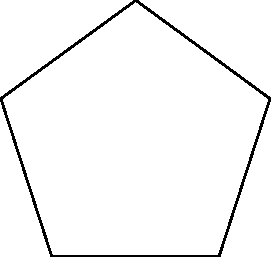
\includegraphics[scale=0.7]{Imatges/figuraE7-3.pdf} 
\end{center}
\noindent
\rule{\textwidth}{3pt}

\begin{center}
\colorbox{black}{\makebox[\textwidth]{  \color{white} {\large {\bfseries Experiment 7-4 (hexàgon regular)}}}}
\end{center}
\index{hexàgon regular, Experiment}
\index{Experiments!hexàgon regular}
{\small
\noindent
Dibuixeu un hexàgon regular utilitzant el mètode \textsf{vegadesRepetir:}.}
\begin{center}
\includegraphics[scale=0.6]{Imatges/figuraE7-4.pdf} 
\end{center}
\noindent
\rule{\textwidth}{3pt}

\vspace*{3mm}

Un cop ho hagueu dominat, intenteu dibuixar un polígon regular amb un nombre molt gran de costats. És possible que hagueu de reduir la mida dels costats per fer que la figura pugui caber a la pantalla. Quan el nombre de costats sigui gran i la mida dels costats sigui petita, el polígon us semblarà un cercle.

\section{Redescobrir les piràmides}
\index{dibuixar!figures geomètriques|)}
\index{figures geomètriques, dibuixar|)}
Recordeu com vau codificar el perfil de la piràmide de Saqqara a l'Experiment 3-5? Podeu simplificar el vostre codi utilitzant un bucle, com a l'\emph{Script}~\ref{scr7-5}.\index{bucles!utilitzar en un \emph{script} per dibuixar una piràmide}
\begin{script}  Un script amb repeticions per dibuixar la piràmide.
\newline
\newline
\noindent
\includegraphics[scale=0.6]{Imatges/figuraS7-5.png}
\noindent
\textsf{\upshape
\begin{tabbing}
\hspace{5mm} \= \kill
$|$ pica $|$\\
pica := Bot nou.\\
5 vegadesRepetir:\\
\>[  pica nord.\\
\>pica ves: 20.\\
\>pica est.\\
\>pica ves: 20  ].\\
5 vegadesRepetir:\\
\>[  pica ves: 20.\\
\>pica sud.\\
\>pica ves: 20.\\
\>pica est  ].\\
pica oest.\\
pica ves: 200.\\
\end{tabbing}
}
\label{scr7-5}
\end{script}

Ara ja hauríeu de generar piràmides amb un nombre arbitrari d'esglaons utilitzant el mateix nombre d'expressions, només canviant els nombres de l'\emph{script}.

\begin{center}
\colorbox{black}{\makebox[\textwidth]{  \color{white} {\large {\bfseries Experiment 7-5 (piràmide amb deu esglaons)}}}}
\end{center}
\index{piràmide amb deu esglaons, Experiment}
\index{Experiments!piràmide amb deu esglaons}
{\small
\noindent
Dibuixeu una piràmide amb 10 esglaons utilitzant una variació de l'\emph{Script}~\ref{scr7-5} .}
\begin{center}
\includegraphics[scale=0.27]{Imatges/figuraE7-5.png} 
\end{center}
\noindent
\rule{\textwidth}{3pt}
\vspace{3mm}

És possible que vulgueu generar piràmides amb un nombre encara més gran d'esglaons. S'hauria d'ajustar la mida dels esglaons si voleu que càpiguen a la pantalla.

\section{Més experiments amb repeticions}
\index{bucles!experimentar amb|(}
Com ja heu comprovat, generar una piràmide esglaonada implica la repetició d'un bloc de codi que dibuixa dos segments de línia. Un cop identifiqueu els elements que cal repetir, podeu produir dibuixos complexos a partir de la repetició de dibuixos elementals. Els experiments següents il·lustren aquest principi.

\begin{center}
\colorbox{black}{\makebox[\textwidth]{  \color{white} {\large {\bfseries Experiment 7-6 (una creu suïssa)}}}}
\end{center}
\index{creu su@una creu su{\"i}ssa, Experiment}
\index{Experiments!creu su@una creu su{\"i}ssa}
{\small
\noindent
Dibuixeu l'esbós de la creu suïssa mostrada a la figura utilitzant \textsf{giraEsquerra:} o bé \textsf{giraDreta:}, i \textsf{vegadesRepetir:}}
\begin{center}
\includegraphics[scale=0.26]{Imatges/figuraE7-6.png} 
\end{center}
\noindent
\rule{\textwidth}{3pt}

\begin{center}
\colorbox{black}{\makebox[\textwidth]{  \color{white} {\large {\bfseries Experiment 7-7 (una escala)}}}}
\end{center}
\index{escala @una escala, Experiment}
\index{Experiments!escala @una escala}
{\small
\noindent
Dibuixeu l'escala que veieu a la figura.}
\begin{center}
\includegraphics[scale=0.72]{Imatges/figuraE7-7.png} 
\end{center}
\noindent
\rule{\textwidth}{3pt}

\begin{center}
\colorbox{black}{\makebox[\textwidth]{  \color{white} {\large {\bfseries Experiment 7-8 (escala sense alçadors)}}}}
\end{center}
\index{escala sense alçadors, Experiment}
\index{Experiments!escala sense alçadors}
{\small
\noindent
Dibuixeu l'escala estilitzada --sense alçadors-- que veieu a la figura.}
\begin{center}
\includegraphics[scale=0.78]{Imatges/figuraE7-8.png} 
\end{center}
\noindent
\rule{\textwidth}{3pt}

\begin{center}
\colorbox{black}{\makebox[\textwidth]{  \color{white} {\large {\bfseries Experiment 7-9 (una grapa)}}}}
\end{center}
\index{grapa @una grapa, Experiment}
\index{Experiments!grapa @una grapa}
{\small
\noindent
Dibuixeu l'element gràfic, semblant a una grapa, mostrat a la figura.}
\begin{center}
\includegraphics[scale=1.4]{Imatges/figuraE7-9.png} 
\end{center}
\noindent
\rule{\textwidth}{3pt}

\begin{center}
\colorbox{black}{\makebox[\textwidth]{  \color{white} {\large {\bfseries Experiment 7-10 (una pinta)}}}}
\end{center}
\index{pinta @una pinta, Experiment}
\index{Experiments!pinta @una pinta}
{\small
\noindent
Transformeu l'element gràfic que heu fet a l'Experiment 7-9 per construir la pinta mostrada a la figura.}
\begin{center}
\includegraphics[scale=0.8]{Imatges/figuraE7-10.png} 
\end{center}
\noindent
\rule{\textwidth}{3pt}
\newpage
\begin{center}
\colorbox{black}{\makebox[\textwidth]{  \color{white} {\large {\bfseries Experiment 7-11 (una escala de mà)}}}}
\end{center}
\index{escala de mà@una escala de mà, Experiment}
\index{Experiments!escala de mà@una escala de mà}
{\small
\noindent
Transformeu l'element gràfic que heu fet a l'Experiment 7-9 per construir una escala de mà.}
\begin{center}
\includegraphics[scale=1.0]{Imatges/figuraE7-11.png} 
\end{center}
\noindent
\rule{\textwidth}{3pt}

\begin{center}
\colorbox{black}{\makebox[\textwidth]{  \color{white} {\large {\bfseries Experiment 7-12 (quadrats que fan tombarelles)}}}}
\end{center}
\index{quadrats que fan tombarelles, Experiment}
\index{Experiments!quadrats que fan tombarelles}
{\small
\noindent
Ara que ja sou uns mestres en repeticions utilitzant \textsf{vegadesRepetir:}, feu un bucle per dibuixar els quadrats fent tombarelles que teniu al començament del capítol~\ref{cap4}. }\\
\noindent
\rule{\textwidth}{3pt}
\index{bucles!experimentar amb|)}

\section{Resum}

En aquest capítol heu après a programar repeticions utilitzant el mètode \textsf{{\itshape n} vegadesRepetir:}.\index{n vegadesRepetir: [], efecte de} \index{vegadesRepetir: mètode!efecte de}

\vspace{5mm}
\noindent
{\small \begin{tabular}{p{22mm}p{45mm}p{38mm}p{28mm}}
\hline
\textbf{Mètode} & \textbf{Sintaxi} & \textbf{Descripció} & \textbf{Exemple}\\
\hline
\textsf{vegadesRepetir:} & \textsf{{\itshape n} vegadesRepetir:\newline \hspace*{5mm} [ {\itshape seqüència d'expressions} ]} &
Repeteix una seqüència \newline d'expressions \emph{n} vegades
& \textsf{10 vegadesRepetir: \newline \hspace*{5mm} [ pica ves: 10. \newline \hspace*{5mm} pica salta: 10 ]} \\
\hline
\end{tabular}}
\index{scripts@\emph{scripts} amb nom|see{mètodes}}

\chapter{Variables}
\label{cap8}

\includegraphics[scale=1.0]{Imatges/figura8-0.png}

Hom sempre posa nom a les coses. Per exemple, donem nom a l'altra gent, als gossos i als cotxes. Quan fem això, estem \emph{associant} algun objecte, ésser o idea amb una paraula o símbol. Un cop hem fet aquesta associació, podem fer servir aquesta paraula per \emph{referir-nos} a o interactuar amb l'objecte associat a ella. Un nom pot durar tota una vida, o el podem descartar després de no gaire temps. Algunes vegades, els noms fan referència a d'altres noms. Per exemple, un actor té usualment diversos noms: el seu nom, el nom d'actor i el nom del personatge que està interpretant. En un llenguatge de programació, també ens cal poder donar nom a les coses, i per a això utilitzem \emph{variables}.

En aquest capítol veureu les variables, que són receptacles per a objectes, i com les podeu utilitzar per simplificar els vostres programes. De fet, les variables són sovint imprescindibles en els programes. Finalment, a mesura que la complexitat dels problemes que anem trobant s'incrementi, veureu que caldrà expressar dependències entre variables. Per exemple, l'amplada d'un rectangle pot ser dos terços de la seva altura. En aquest capítol us mostrarem com fer servir les variables per expressar dependències entre diverses quantitats.

\section{Per cortesia de la lletra A}
\index{A!forma de}
\index{lletra A!forma de}
Tal com vau fer al capítol~\ref{cap3}, imagineu que voleu utilitzar un robot per escriure lletres de l'alfabet. La lletra A més aviat primitiva que dibuixarem tot seguit està caracteritzada per la seva \emph{altura}, la seva \emph{amplada} i la seva \emph{mitja altura}, que és l'altura a què dibuixem la línia del mig de la lletra A (figura~\ref{fig0801}). \index{altura, variable; relació amb l'amplada i la mitja altura} \index{mitja altura, variable; relació amb l'amplada i l'altura} \index{amplada, variable; relació amb l'altura i la mitja altura}
\begin{figure}[h]
\begin{center}
\includegraphics[scale=0.25]{Imatges/figura8-1.pdf}
\end{center}
\caption{La forma de la lletra A es caracteritza per la seva altura, la seva amplada i la seva mitja altura.}
\label{fig0801}
\end{figure}

\begin{center}
\colorbox{black}{\makebox[\textwidth]{  \color{white} {\large {\bfseries Experiment 8-1}}}}
\end{center}
{\small
\noindent
Feu un \emph{script} que dibuixi una lletra A d'altura 100 píxels, amplada 70 píxels i mitja altura 60 píxels}\\
\noindent
\rule{\textwidth}{3pt}

\subsection{Variacions sobre el tema de la A}
\index{A!variacions|(}
\index{lletra A!variacions|(}

L'\emph{script} que heu escrit per a l'Experiment 8-1 s'hauria d'assemblar a l'\emph{Script}~\ref{scr8-1}.

\begin{script}  Una A per a l'Experiment 8-1
\textsf{\upshape
\\
\\$|$ pica $|$\\
pica := Bot nou.\\
pica nord.\\
pica ves: 100.\\
pica est.\\
pica ves: 70.\\
pica sud.\\
pica ves: 100.\\
pica oest.\\
pica salta: 70.\\
pica nord.\\
pica ves: 60.\\
pica est.\\
pica ves: 70.\\
}
\label{scr8-1}
\end{script}

\begin{center}
\colorbox{black}{\makebox[\textwidth]{  \color{white} {\large {\bfseries Experiment 8-2 (frAnkenstein)}} }}
\end{center}
\index{frAnkenstein, Experiment}
\index{Experiments!frAnkenstein}
{\small
\noindent
Modifiqueu l'\emph{Script}~\ref{scr8-1} per dibuixar una lletra A monstruosa d'altura 200 píxels, amplada 100 píxels i mitja altura 70 píxels, com veieu a la figura.}
\begin{center}
\includegraphics[scale=3.0]{Imatges/figuraE8-2.png}
\end{center}
\noindent
\rule{\textwidth}{3pt}
\vspace{3mm}

En modificar l'\emph{Script}~\ref{scr8-1} per a l'Experiment 8-2, heu vist que per fer una A de mida diferent, heu hagut de canviar els valors que representen l'altura, l'amplada i la mitja altura de la lletra \emph{a tot arreu} on aquests nombres apareixen, i a més ho heu hagut de fer \emph{síncronament}. Per síncronament volem dir ``en l'ordre correcte''; és a dir, el 100 hauria de ser un 200, el 70 hauria de ser un 100 i el 60 hauria de ser un 70, sense barrejar-los.
\begin{center}
\colorbox{black}{\makebox[\textwidth]{  \color{white} {\large {\bfseries Experiment 8-3}}}}
\end{center}
{\small
\noindent
Modifiqueu l'\emph{Script}~\ref{scr8-1} per dibuixar altres A de mides diferents. Proveu de reproduir algunes de les As que apareixen a la figura del començament d'aquest capítol.}\\
\noindent
\rule{\textwidth}{3pt}
\vspace{1mm}

Fent l'Experiment 8-3 heu arribat sens dubte a la conclusió que canviar els valors de les característiques de la lletra A a tot arreu és força avorrit. És més, hauria de ser obvi que fent aquests canvis us arrisqueu a confusions, a oblidar algun valor o a fer un canvi de valor incorrecte. El resultat no serà gens semblant al que teniu al cap quan feu l'\emph{script}. Podeu imaginar que en programes complexos, canviar els valors un per un tal com ho heu fet pot ser força problemàtic.
\index{A!variacions|)}
\index{lletra A!variacions|)}

\section{Variables al rescat}
\index{expressió d'assignació (:=)!utilitzar en variables|(}
\index{variables!inicialitzar|(}
Fer molts canvis per construir lletres de diverses mides i formes és molt pesat i pot introduir errors. Ens cal una solució que ens estalviï barrejar els nombres que representen les diferentes característiques d'una lletra i que també ens permeti fer alteracions sense haver de canviar els valors a tot arreu. De fet, voldríem ser capaços de fer el següent:
\begin{itemize}
\item \emph{Declarar} l'altura, l'amplada i la mitja altura de la lletra A només un cop a tot l'\emph{script}.
\item \emph{Referir-nos} a aquests valors si els necessitem.
\item \emph{Canviar} els valors, si cal.
\end{itemize}

Aquestes tres coses són exactament el que una variable ens permet fer!  Fantàstic, no? Una variable és un \emph{nom} a què \emph{associem un valor}. Cal \emph{declarar} la variable i \emph{associar-li} un valor nou. Aleshores podrem \emph{referir-nos} a la variable i obtenir-ne el valor. També és possible \emph{modificar} el valor associat a la variable i assignar-li un valor nou. El valor d'una variable pot ser un nombre, una col·lecció d'objectes, o fins i tot un robot. Tot seguit mostrarem com declarar, associar un valor i utilitzar una variable. \index{variables!definir}
\newpage
\noindent
\rule{\textwidth}{2pt}
\noindent
\textbf{Important!}  Una variable és un \emph{nom} a què \emph{associem un valor}. Cal que \emph{declarem} la variable i li \emph{associem} un valor nou. Aleshores podrem \emph{referir-nos} a la variable i obtenir-ne el valor. També és possible \emph{modificar} el valor associat a la variable i associar-hi un valor nou. \\
\noindent
\rule{\textwidth}{2pt}

\subsection{Declarar una variable}
\index{variables!declarar}
\index{\textbar\textbar (barres verticals) posar variables entre}
\index{barres verticals (\textbar\textbar) posar variables entre}
Abans d'utilitzar una variable, l'hem de \emph{declarar}; és a dir, li hem de dir a Squeak el nom de la variable que volem fer servir. Declarem variables posant-les entre barres verticals $|$ $|$, com veieu en l'exemple, que declara tres variables \textsf{altura}, \textsf{amplada} i \textsf{mitjaAltura}:

\noindent
\textsf{ 
\\
$|$ altura amplada mitjaAltura $|$}
\vspace{3mm}

\noindent
Per ser precís, les barres verticals \textbar \hspace*{2mm} \textbar declaren variables \emph{temporals}, que són variables que existeixen només mentre s'executa l'\emph{script}.\index{variables!inicialitzar|)}

\subsection{Assignar un valor a una variable}
\index{variables!assignar valors a}
\index{valors!assignar a variables}
\index{valors!relació amb les variables}
\index{:= (expressió d'assignació)!utilitzar en variables|(}
Abans de fer servir una variable és quasi sempre necessari donar-li un valor. Associar un valor a una variable s'anomena \emph{assignar} un valor a una variable. Smalltalk utilitza el símbol (compost per un parell de caràcters) \textsf{:=} per assignar un valor a una variable. A l'\emph{script} següent, després de declarar tres variables, assignem \textsf{100} a la variable \textsf{altura}, \textsf{70} a la variable \textsf{amplada} i \textsf{60} a la variable \textsf{mitjaAltura}. Quan assignem un valor a una variable per primera vegada, diem que la \emph{inicialitzem}:

\noindent
\textsf{ 
\\
$|$ altura amplada mitjaAltura $|$\\
altura := 100.\\
amplada := 70.\\
mitjaAltura := 60.\\
}

\vspace{3mm}
\noindent
\rule{\textwidth}{2pt}
\noindent
\textbf{Important!}  El símbol \textsf{:=} assigna un valor a una variable. Per exemple, \textsf{altura := 120} assigna el valor \textsf{120} a la variable \textsf{altura}, mentre que \textsf{longitud := 120 + 30} assigna el resultat de l'expressió \textsf{120 + 30}, és a dir, \textsf{150}, a la variable \textsf{longitud}

\noindent
\rule{\textwidth}{2pt}

\noindent
Quan assignem un valor a una variable per primer cop, diem que l'estem \emph{inicialitzant}.

\noindent
\rule{\textwidth}{2pt}

\subsection{Referir-nos a les variables}
\index{variables!referir-nos a les}
\index{expressió d'assignació (:=)!utilitzar en variables|)}
\index{:= (expressió d'assignació)!utilitzar en variables|)}
Per referir-nos al valor assignat a una variable --també parlem d'\emph{utilitzar} una variable-- senzillament escrivim el seu nom. Al següent \emph{script}, després d'haver \emph{declarat} les variables a la primera línia, la variable \textsf{altura} s'\emph{inicialitza} amb el valor \textsf{100} a  la línia 3 i s'\emph{utilitza} a la línia 5 per dir-li al robot que vagi endavant el nombre de píxels associat amb la variable \textsf{altura}, que aquí és \textsf{100}.

\noindent
\textsf{ 
\\
$|$ pica altura $|$\\
pica := Bot nou.\\
altura := 100.\\
pica nord.\\
pica ves: {\bfseries altura}.
}


\vspace{3mm}
\noindent
\rule{\textwidth}{2pt}
\noindent
\textbf{Important!}  En general, cal \emph{declarar} i \emph{inicialitzar} una variable abans d'utilitzar-la.

\noindent
\rule{\textwidth}{2pt}

\subsection{I què passa amb Pica?}
\index{pica, robot!com a variable}
Ho heu encertat! \textsf{pica} també és una variable. El que passa és que el seu valor és un robot. Per tant, \textsf{$|$ pica $|$} declara una variable anomenada \textsf{pica}. L'expressió \textsf{pica := Bot nou} inicialitza la variable amb un valor, que aquí és un robot nou. Aleshores utilitzem aquest robot tot enviant-li missatges via la variable \textsf{pica}, per exemple, \textsf{pica ves: 100}.

\section{Utilitzar variables}
\index{A!utilitzar variables|(}
\index{lletra A!utilitzar variables|(}
\index{variables!utilitzar en la lletra A|(}
Ara explorarem els beneficis d'utilitzar variables, i us mostrarem algunes propietats interessants de les variables. En particular, us ensenyarem la potència que aconseguim en expressar relacions entre variables.

Introduint variables a  l'\emph{Script}~\ref{scr8-1}, obtenim  l'\emph{Script}~\ref{scr8-2}
\begin{script}  Una A amb variables.
\textsf{\upshape
\begin{tabbing}
\hspace{50mm} \= \kill
$|$ pica {\bfseries altura amplada mitjaAltura} $|$\\
pica := Bot nou.\\
{\bfseries altura := 100.} \> {\itshape ``inicialitzem les variables''}\\
{\bfseries amplada := 70.}\\
{\bfseries mitjaAltura := 60.}\\
pica nord.\\
pica ves: {\bfseries altura.} \> {\itshape ``després utilitzem les variables''}\\
pica est.\\
pica ves: {\bfseries amplada.}\\
pica sud.\\
pica ves: {\bfseries altura.}\\
pica oest.\\
pica salta: {\bfseries amplada.}\\
pica nord.\\
pica ves: {\bfseries mitjaAltura.}\\
pica est.\\
pica ves: {\bfseries amplada.}
\end{tabbing}
}
\label{scr8-2}
\end{script}

Estareu d'acord que canviar els valors de les variables una vegada és més senzill que canviar els nombres repartits per tot l'\emph{script}. Canvieu alguns valors, així us n'acabareu de convèncer. Hauríeu de ser capaços de dibuixar totes les A de la figura
del començament del capítol. Ara, si voleu canviar les característiques de la vostra A, només us cal re-inicialitzar les variables tot canviant els valors a les línies 3, 4 i 5, com veieu a l'\emph{Script}~\ref{scr8-3}. El dibuix resultant us el mostrem a la figura~\ref{fig0802}.
\begin{script}  Una lletra A modificada.
\textsf{\upshape
\begin{tabbing}
\hspace{50mm} \= \kill
$|$ pica {\bfseries altura amplada mitjaAltura} $|$\\
pica := Bot nou.\\
{\bfseries altura := 30.} \> {\itshape ``inicialitzem les variables''}\\
{\bfseries amplada := 200.}\\
{\bfseries mitjaAltura := 10.}\\
\dots
\end{tabbing}
}
\label{scr8-3}
\end{script}
\begin{figure}[h]
\begin{center}
\includegraphics[scale=2.0]{Imatges/figura8-2.png}
\end{center}
\caption{Una A curta i ampla creada simplement inicialitzant \textsf{\upshape altura := 30}, \textsf{\upshape amplada := 200} i \textsf{\upshape mitjaAltura := 10}.}
\label{fig0802}
\end{figure}

Utilizant variables podeu crear fàcilment moltes lletres diferents, i en un futur podreu escriure programes per resoldre molts problemes interessants. Tornem un moment enrere i considerem la potència que ens proporcionen les variables. \index{A!utilitzar variables|)} \index{lletra A!utilitzar variables|)} \index{variables!utilitzar en la lletra A|)}

\subsection{La potència de les variables}
\index{variables!potencia@potència de|(}
Els experiments que trobareu en el que queda de capítol il·lustren la potència de les variables. Les variables us permeten donar nom a una entitat, ja sigui un robot, una longitud o pràcticament qualsevol altra cosa. Després podeu utilitzar els noms en lloc de repetir els valors que heu associat amb aquests noms. Les variables fan que els vostres \emph{scripts} siguin molt més senzills de canviar, ja que només cal re-inicialitzar les variables amb valors diferents.

A més a més, una variable pot contenir una gran varietat de tipus de valors. Fins ara, heu assignat robots i nombres a les variables, però també podeu assignar colors (per exemple, \textsf{robotColor := Color groc}), sons, o qualsevol objecte d'Squeak.

Fixeu-vos també que les variables fan els vostres \emph{scripts} més llegibles i fàcils d'entendre. Per quedar-ne convençuts, compareu l'\emph{Script}~\ref{scr8-1} i l'\emph{Script}~\ref{scr8-2}. El fet d'utilitzar variables amb noms com ``altura'' o ``amplada'' us ajuda a entendre com es dibuixa la lletra. \index{variables!potencia@potència de|)}

\subsection{Expressar les relacions entre variables}
\index{variables!expressar relacions entre|(}
En els vostres experiments amb la lletra A, segurament heu trobat que algunes de les lletres són més reconeixibles que altres. Les lletres de l'alfabet haurien de mantenir certes proporcions per ser llegibles. En particular, les dimensions que descriuen una lletra concreta no es trien a l'atzar, sinó que existeixen unes certes proporcions.

Podem decidir, per a la nostra lletra A, que l'amplada hauria de ser dos terços de l'altura, i que la mitja altura hauria de ser tres cinquenes parts de l'altura. Podem expressar aquestes relacions utilitzant variables com ensenyem a l'\emph{Script}~\ref{scr8-4}. Com podeu veure, el valor d'una variable no ha de ser un simple nombre, sinó que pot ser el resultat d'algun càlcul complex.
\begin{script}  Relacions entre variables: una primera aproximació.
\textsf{\upshape
\begin{tabbing}
\hspace{50mm} \= \kill
$|$ pica altura amplada mitjaAltura $|$\\
pica := Bot nou.\\
altura := {\bfseries 120.}\\
amplada := {\bfseries 120} * 2 / 3.\\
mitjaAltura := {\bfseries 120} * 3 / 5.\\
\dots
\end{tabbing}
}
\label{scr8-4}
\end{script}

Mirant l'\emph{Script}~\ref{scr8-4}, aviat us adoneu que no és òptim. Les relacions entre les variables no s'expressen entre les variables, sinó en termes del valor \textsf{120} (a les línies 3, 4 i 5). Aquest valor hauria de ser canviat manualment si volguéssiu fer una altra lletra A amb les mateixes proporcions. Vosaltres voleu ser capaços de canviar el valor d'\textsf{altura} i que els valors d'\textsf{amplada} i \textsf{mitjaAltura} canviïn automàticament. La solució està a utilitzar la variable \textsf{altura} en lloc del valor \textsf{120}, com veieu a l'\emph{Script}~\ref{scr8-5}. En aquest \emph{script}, els valors de les variables \textsf{amplada} i \textsf{mitjaAltura} realment depenen del valor d'\textsf{altura}. Això funciona ja que el valor d'una variable pot ser expressat en termes d'altres variables. L'expressio \textsf{amplada := altura * 2 / 3} expressa que l'amplada de la lletra és igual a dos terços de la seva altura.
\begin{script}  Relacions entre variables: Les variables \textsf{{\upshape amplada}} i \textsf{{\upshape mitjaAltura}} depenen d'\textsf{{\upshape altura}}.
\textsf{\upshape
\begin{tabbing}
\hspace{50mm} \= \kill
$|$ pica altura amplada mitjaAltura $|$\\
pica := Bot nou.\\
{\bfseries altura := 120.}\\
amplada := {\bfseries altura} * 2 / 3.\\
mitjaAltura := {\bfseries altura} * 3 / 5.\\
pica nord.\\
\dots
\end{tabbing}
}
\label{scr8-5}
\end{script}

\vspace*{2mm}

\noindent
{\large Inicialitzeu abans d'utilitzar!}
\vspace*{5mm}

\noindent
L'única restricció que heu de considerar en expressar relacions entre variables és que una variable utilitzada a la definició d'una altra variable hauria de tenir un valor. Per exemple, a l'\emph{Script}~\ref{scr8-5}, la variable \textsf{altura} té \textsf{120} com a valor d'inicialització, que és utilitzat per \textsf{amplada} i \textsf{mitjaAltura} en calcular els seus valors inicials. Per veure què pot anar malament, a l'\emph{Script}~\ref{scr8-6} la variable \textsf{altura} no ha estat inicialitzada, i per tant quan provem d'inicialitzar la variable \textsf{amplada} a \textsf{altura * 2 / 3} obtenim un error ja que \textsf{altura} no té cap valor. Parlarem més sobre els errors al capítol~\ref{cap15}. \index{variables!expressar relacions entre|)}
\begin{script}  Inicialització problemàtica d'\textsf{{\upshape amplada}}.
\textsf{\upshape
\begin{tabbing}
\hspace{50mm} \= \kill
$|$ altura amplada mitjaAltura $|$\\
amplada := altura * 2 / 3.\\
altura := 120.\\
mitjaAltura :=  altura * 3 / 5.
\end{tabbing}
}
\label{scr8-6}
\end{script}

\section{Experimentar amb variables}
\index{variables!experimentar amb|(}
Els experiments que segueixen us ajudaran a guanyar experiència amb les variables.

\begin{center}
\colorbox{black}{\makebox[\textwidth]{  \color{white} {\large {\bfseries Experiment 8-4 (el rectangle d'or)}} }}
\end{center}
\index{rectangle d'or@el rectangle d'or, Experiment}
\index{Experiments!rectangle d'or@el rectangle d'or}
\index{scripts@\emph{scripts}!pel rectangle d'or}
{\small
\noindent
Un rectangle d'or és un rectangle tal que un dels seus costats és aproximadament 1.6 vegades la longitud de l'altre. El nombre 1.6 és una aproximació de la ``raó àuria'': el nombre. Una propietat interessant d'aquests rectangles és que si talleu un quadrat del rectangle, com veieu a la figura, el rectangle que queda també és un rectangle d'or. Ara podeu tallar un quadrat d'aquest rectangle més petit i obtenir un rectangle d'or encara més petit, i així \emph{ad infinitum}. Les dimensions d'un rectangle d'or són agradables a la vista, i des de temps antics, artistes i arquitectes han utilitzat la raó àuria a la seva feina. Feu un \emph{script} que dibuixi un rectangle d'or. Podeu expressar el nombre en Smalltalk de la forma \textsf{1 + 5 sqrt / 2}}
\begin{center}
\includegraphics[scale=2.5]{Imatges/figuraE8-4.png}
\end{center}
\noindent
\rule{\textwidth}{3pt}

\begin{center}
\colorbox{black}{\makebox[\textwidth]{  \color{white} {\large {\bfseries Experiment 8-5 (\emph{Scripts} que no funcionen)}} }}
\end{center}
\index{scripts que no@\emph{Scripts} que no funcionen, Experiment}
\index{Experiments!scripts que no@\emph{Scripts} que no funcionen}
{\small
\noindent
Expliqueu per quina raó cap dels \emph{scripts} següents és capaç de dibuixar una lletra A d'altura 120 píxels.}
\begin{multicols}{2}{

\noindent
\textsf{\upshape
$|$ pica altura $|$\\
pica := Bot nou.\\
altura := 120.\\
pica nord.\\
pica ves: 100.\\
pica est.\\
pica ves: 70.\\
pica sud.\\
pica ves: 100.\\
pica oest.\\
pica salta: 70.\\
pica nord.\\
pica ves: 50.\\
pica est.\\
pica ves: 70.
}
\columnbreak

\noindent
\textsf{\upshape
$|$ pica altura $|$\\
pica := Bot nou.\\
pica nord.\\
pica ves: altura.\\
pica est.\\
pica ves: 70.\\
pica sud.\\
pica ves: altura.\\
pica oest.\\
pica salta: 70.\\
pica nord.\\
pica ves: 50.\\
pica est.\\
pica ves: 70.\\
}
}
\end{multicols}

\noindent
\rule{\textwidth}{3pt}

\subsection{Les piràmides redescobertes}

A l'\emph{Script}~\ref{scr7-5}, al capítol~\ref{cap7}, vam definir el perfil de la piràmide de Saqqara com a l'\emph{Script}~\ref{scr8-7}.
\begin{script}  La piràmide de Saqqara.
\newline
\newline
\noindent
\includegraphics[scale=0.6]{Imatges/figuraS8-7.png}
\noindent
\textsf{\upshape
\begin{tabbing}
\hspace{5mm} \= \kill
$|$ pica $|$\\
pica := Bot nou.\\
5 vegadesRepetir:\\
\>[  pica nord.\\
\>pica ves: 20.\\
\>pica est.\\
\>pica ves: 20  ].\\
5 vegadesRepetir:\\
\>[  pica ves: 20.\\
\>pica sud.\\
\>pica ves: 20.\\
\>pica est  ].\\
pica oest.\\
pica ves: 200.\\
\end{tabbing}
}
\label{scr8-7}
\end{script}

\begin{center}
\colorbox{black}{\makebox[\textwidth]{  \color{white} {\large {\bfseries Experiment 8-6 (una piràmide amb un nombre variable d'esglaons)}}}}
\end{center}
\index{piràmide amb un nombre@una piràmide amb un nombre variable d'esglaons, Experiment}
\index{Experiments!piràmide amb un nombre@una piràmide amb un nombre variable d'esglaons}
\index{nombreEsglaons variable, utilitzar en piràmide}
{\small
\noindent
Modifiqueu l'\emph{Script}~\ref{scr7-5}, introduint la variable \textsf{nombreEsglaons} per representar el nombre d'esglaons que hauria de tenir  la piràmide.}\\
\noindent
\rule{\textwidth}{3pt}
\begin{center}
\colorbox{black}{\makebox[\textwidth]{  \color{white} {\large {\bfseries Experiment 8-7 (una piràmide amb una mida variable de l'esglaó)}}}}
\end{center}
\index{piràmide amb una mida@una piràmide amb una mida variable de l'esglaó, Experiment}
\index{Experiments!piràmide amb una mida@una piràmide amb una mida variable de l'esglaó}
\index{midaEsglaons variable, utilitzar en piràmide}
\index{variables!utilitzar en l'Experiment de la piràmide de Saqqara}
{\small
\noindent
Modifiqueu l'\emph{Script} de l'Experiment 8-6 introduint la variable \textsf{midaEsglaons} per representar la mida dels esglaons.}\\
\noindent
\rule{\textwidth}{3pt}

\section{Polígons automatitzats utilitzant variables}
\index{variables!experimentar amb|)}
\index{variables!automatitzar polígons amb|(}
\index{poligon@polígon!automatitzar amb variables|(}
La utilització de variables simplifica enormement la definició d'\emph{scripts} on alguna de les \emph{variables} depèn d'altres variables. En aquesta secció, veureu com l'ús de variables proporciona força avantatges a l'hora de tractar amb bucles. El capítol~\ref{cap10} aprofundirà més en la potència que la combinació de variables i bucles proporciona als vostres programes.

Tornem als Experiments 7-3 i 7-4, en què un \textsf{Bot} havia de dibuixar un pentàgon regular i un hexàgon regular. El codi necessari apareix aquí com a \emph{Scripts}~\ref{scr8-8} i~\ref{scr8-9}.\index{hexàgons!exemple de} \index{pentàgon, exemple de} \index{hexàgon regular, exemple de} \index{pentàgon regular, exemple de}
\begin{script}  Un pentàgon regular.
\newline
\newline
\noindent
\includegraphics[scale=0.6]{Imatges/figuraS8-8.pdf}
\noindent
\textsf{\upshape
\begin{tabbing}
\hspace{5mm} \= \kill
$|$ pica $|$\\
pica := Bot nou.\\
5 vegadesRepetir:\\
\>[  pica ves: 100.\\
\>pica giraEsquerra: 72  ].\\
\end{tabbing}
}
\label{scr8-8}
\end{script}
\begin{script}  Un hexàgon regular.
\newline
\newline
\noindent
\includegraphics[scale=0.5]{Imatges/figuraS8-9.pdf}
\noindent
\textsf{\upshape
\begin{tabbing}
\hspace{5mm} \= \kill
$|$ pica $|$\\
pica := Bot nou.\\
6 vegadesRepetir:\\
\>[  pica ves: 100.\\
\>pica giraEsquerra: 60  ].\\
\end{tabbing}
}
\label{scr8-9}
\end{script}

Per transformar el primer \emph{script} en el segon només cal canviar el nombre de costats (diguem-ne $s$) \emph{i} el gir (diguem-ne $T$) de manera que el producte $s \times T$ sigui igual a 360. No estaria bé poder escriure un \emph{script} on només calgués canviar un nombre, diguem-ne el nombre de costats, ja que aquest és el paràmetre més senzill? Això ho podem fer mitjançant les variables. Proveu de trobar-ne una solució. \index{variable angle!utilització amb polígons}

L'\emph{Script}~\ref{scr8-10} resol el problema. Fa possible dibuixar un polígon regular amb qualsevol nombre de costats, només canviant un nombre. Proveu-lo abans de continuar la discussió.\index{costats variable, utilitzar en polígons}
\begin{script}  Dibuixar un polígon regular.
\textsf{\upshape
\begin{tabbing}
\hspace{5mm} \= \kill
$|$ pica costats angle $|$\\
pica := Bot nou.\\
costats := 6.\\
angle := 360 / costats.\\
costats vegadesRepetir:\\
\> [ pica ves: 100.\\
\> pica giraEsquerra: angle].\\
\end{tabbing}
}
\label{scr8-10}
\end{script}

Aquest \emph{script} introdueix dues noves variables, \textsf{costats} i \textsf{angle}, que s'utilitzen per guardar el nombre de costats i l'angle.
Aleshores, l'expressió \textsf{costats := 6} assigna el valor \textsf{6} a la variable \textsf{costats}, i l'expressió \textsf{angle := 360 / costats} assigna un valor a la variable \textsf{angle} que és el resultat de dividir 360 pel valor contingut a la variable \textsf{costats}. El valor de la variable \textsf{angle} s'utilitza com a argument del missatge \textsf{giraEsquerra:} enviat al robot dins del bloc que es repeteix. \index{poligon@polígon!automatitzar amb variables|)} \index{variables!automatitzar polígons amb|)}

\section{Polígons regulars de mida fixa}
\index{poligon@polígon!de mida fixa}
Segur que us heu adonat que si l'\emph{Script}~\ref{scr8-10} s'executa amb un nombre molt gran de costats, la figura no cap a la pantalla.
El proper experiment us demana que arregleu aquest problema reduint la longitud dels costats a mesura que creix el nombre de costats.

\begin{center}
\colorbox{black}{\makebox[\textwidth]{  \color{white} {\large {\bfseries Experiment 8-8 (controlar els costats del polígon)}} }}
\end{center}
\index{controlar els costats del polígon, Experiment}
\index{Experiments!controlar els costats del polígon}
\index{poligon regular@polígon regular!de mida fixa}
\index{longitudTotal variable, utilitzar en polígons}
{\small
\noindent
Modifiqueu l'\emph{Script}~\ref{scr8-10} de manera que la mida del polígon regular romangui més o menys constant mentre canvia el nombre de costats. Ajuda: Introduïu una variable \textsf{longitudTotal} que s'inicialitza a un valor determinat fix, i feu que cada costat del polígon tingui longitud igual a \textsf{longitudTotal} dividit pel nombre de costats.}
\begin{center}
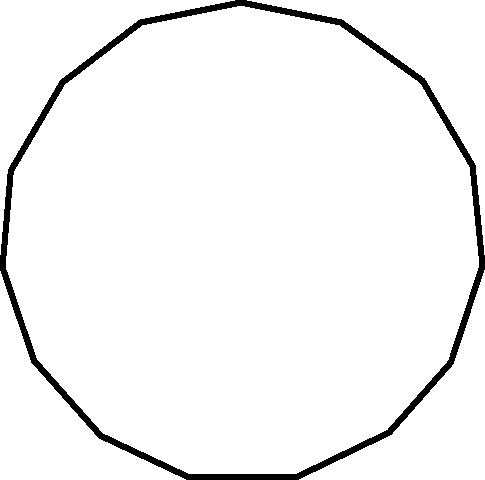
\includegraphics[scale=0.5]{Imatges/figuraE8-8.pdf}
\end{center}
\noindent
\rule{\textwidth}{3pt}

\section{Resum}

\begin{itemize}
\item Una variable és un \emph{nom} a què podem \emph{associar un valor}. Les variables han de ser \emph{declarades} i cal que els \emph{assignem} un valor. Aleshores, podem \emph{referir-nos} a la variable per obtenir-ne el \emph{valor} associat. També és possible \emph{modificar} el valor associat a una variable i assignar-hi un nou valor. 
\item Una variable pot ser utilitzada a qualsevol lloc on el seu valor pugui ser utilitzat.
\item El primer cop que assignem un valor a una variable, diem que la \emph{inicialitzem}.
\item El símbol \textsf{:=} assigna un valor a una variable. Per exemple, \textsf{altura := 120} assigna el valor \textsf{120} a la variable \textsf{altura}, mentre que \textsf{longitud := 120 + 30} assigna el resultat de l'expressió \textsf{120 + 30}, és a dir, \textsf{150}, a la variable \textsf{longitud}.
\item Una variable ha de ser, en general, \emph{declarada} i \emph{inicialitzada} abans de ser utilitzada.
\end{itemize}
\index{variables!declarar i assignar}

\vspace*{5mm}
\noindent
\setlength{\extrarowheight}{1mm}
{\small \begin{tabular}{p{30mm}p{30mm}p{40mm}p{30mm}}
\hline
\textbf{Ús de la variable} & \textbf{Sintaxi} & \textbf{Descripció} & \textbf{Exemple}\\
\hline
declaració de \newline variables & \textsf{$|$ {\itshape nomVariable} $|$} &
Declarar \textsf{nomVariable} com a variable.
& \textsf{$|$ pica altura $|$}\\
assignació de \newline variables & \textsf{{\itshape nomVar} := {\itshape expressió}} &
Assignar el valor d'\textsf{{\itshape expressió}} a la variable \textsf{{\itshape nomVar}}
& \textsf{longitud := 40  \newline  longitud := 30 + 20}\\ 
&  &
Utilitzar el nom d'una variable en una expressió.
& \textsf{pica ves: longitud}\\ 
&  &
Canviar el valor d'una variable utilitzant el seu valor actual.
& \textsf{long := long + 10}\\ 
\hline
\end{tabular}}

\chapter{Aprofundir en les variables}
\label{cap9}

En el capítol anterior vam introduir les variables. En aquest capítol aprofundirem en el tema de manera que pugueu aprendre més sobre com s'utilitzen les variables. Podeu optar per ometre aquest capítol en una primera lectura, ja que és una mica tècnic.

Abans d'il·lustrar amb detalls com funcionen les variables, voldríem posar èmfasi altre cop en la importància de triar noms adequats per a  les variables.

\section{Anomenar les variables}
\index{Smalltalk!anomenar les variables}
\index{variables!anomenar}
En triar un nom per a una variable, podeu triar el nom que vulgueu. Tot i així, és molt important donar a les vostres variables noms amb un cert significat, ja que això us ajudarà a escriure programes i a entendre els programes que ja heu escrit. Per il·lustrar-ho, llegiu l'\emph{Script}~\ref{scr9-1}, que és l'\emph{Script}~\ref{scr8-10} escrit utilitzant noms de variables sense cap significat.
\begin{script}  Les variables sense cap significat fan que un programa sigui difícil d'entendre.
\textsf{\upshape
\begin{tabbing}
\hspace{5mm} \= \kill
$|$ x y z $|$\\
x := Bot nou.\\
y := 6.\\
z := 360 / y.\\
y vegadesRepetir:\\
\> [ x ves: 100.\\
\> x giraEsquerra: z].\\
\end{tabbing}
}
\label{scr9-1}
\end{script}

Com podeu descobrir tot provant-lo, l'\emph{Script}~\ref{scr9-1} és perfectament correcte, i Squeak pot executar-lo sense cap problema. Però estem segurs que teniu clar quin dels dos \emph{Scripts}~\ref{scr8-10} i~\ref{scr9-1} és més comprensible.

A Smalltalk el nom d'una variable pot ser qualsevol seqüència de caràcters alfabètics i numèrics (\emph{alfanumèrics}) començant per una lletra minúscula. És habitual utilitzar noms de variable llargs que indiquen clarament quina funció té la variable dins del programa. Fent-ho així us ajuda, a vosaltres i a d'altres programadors, a entendre millor els vostres \emph{scripts}.

Ser capaç d'entendre el que fa un programa és molt important, ja que, com veureu més tard, un programa usualment implica una combinació de diversos \emph{scripts}\footnote{Això és una simplificació. Aviat sabreu més coses sobre els mètodes, que són els autèntics fonaments de la programació amb objectes}. Quan arribi el moment d'entendre un \emph{script} escrit per algú altre, o fins i tot un d'escrit per vosaltres mateixos fa temps, estareu agraïts d'haver agafat l'hàbit de triar noms de variables significatius.\index{variable, nom de!importància}

Ara que ja us hem convençut de la importancia de triar els noms de les variables amb significat, discutirem en detall les variables.

\section{Variables com a contenidors}
\index{variables!contenidors@com a contenidors|(}
\index{contenidors!variables com a|(}
\index{pica, variable; declarar|(}
Les variables són receptacles que fan referència als objectes. Una manera habitual d'explicar la noció de variable és utilitzar una notació gràfica en què les variables es representen com a contenidors. Veiem aquesta idea a l'\emph{Script}~\ref{scr9-2} i la figura~\ref{fig0901}.

A l'\emph{Script}~\ref{scr9-2} (pas (a) a l'\emph{script} i a la figura), dues variables han estat declarades, \textsf{pica} i \textsf{pablo}. Al pas (b) creem un robot i l'assignem a la variable \textsf{pica}; és a dir, la variable \textsf{pica} ara fa referència al robot que tot just hem creat. Després, a (c), assignem el valor de la variable \textsf{pica} a la variable \textsf{pablo}, i per tant \textsf{pablo} fa referència (també es diu \emph{apunta}) al mateix objecte a què apunta la variable \textsf{pica}, el robot que acabem de crear. Quan enviem un missatge utilitzant qualsevol de les dues variables, estem enviant un missatge al mateix objecte, és a dir, al robot creat al pas (b), ja que les dues variables fan referència al mateix objecte. Per tant, a (d), el missatge enviat a \textsf{pica} fa que el robot es mogui 100 píxels, mentre que l'enviament de missatge (e), que va dirigit a \textsf{pablo}, fa que \emph{el mateix} robot canviï el seu color a groc.\index{pablo, variable; declarar|(}

Una altra manera de pensar això és considerar que el robot té dos noms: \textsf{pica} i \textsf{pablo}. És tot just com si la mare de l'artista Pablo Picasso hagués dit ``Picasso, vine aquí'' (\textsf{pica ves: 100}), i després hagués dit ``Pablo, aquí tens la teva camisa groga. Posa-te-la'' (\textsf{pablo color: Color groc}).
\begin{script}  Dues variables apunten al mateix robot.
\textsf{\upshape
\begin{tabbing}
\hspace{10mm} \= \kill
(a) \> $|$ pica pablo $|$\\
(b) \> pica := Bot nou.\\
(c) \> pablo := pica.\\
(d) \> pica ves: 100.\\
(e) \> pablo color: Color groc.\\
\end{tabbing}
}
\label{scr9-2}
\end{script}
\begin{figure}[h]
\begin{center}
\includegraphics[scale=0.225]{Imatges/figura9-1.pdf}
\end{center}
\caption{
\textbf{\upshape (a)} Dues variables són declarades, \textsf{\upshape pica} i \textsf{\upshape pablo}.
\textbf{\upshape (b)} Es crea un robot i la variable \textsf{\upshape pica} s'associa amb aquest objecte nou.
\textbf{\upshape (c)} S'assigna a la variable \textsf{\upshape pablo} el valor de la variable \textsf{\upshape pica}; ara \textsf{\upshape pablo} apunta al mateix objecte que apunta \textsf{\upshape pica}.
\textbf{\upshape (d)} Quan enviem el missatge \textsf{\upshape ves: 100} utilitzant \textsf{\upshape pica}, el robot es mou.
\textbf{\upshape (e)} Quan enviem el missatge \textsf{\upshape color: Color groc} a \textsf{\upshape pablo}, el mateix robot canvia de color.
Resumint, si enviem un missatge a qualsevol de les dues variables, estem enviant aquest missatge al mateix objecte
}
\label{fig0901}
\end{figure}

\vspace*{5mm}

\section{Assignació: L'esquerra i la dreta de :=}
\index{pablo, variable; declarar|)}
\index{contenidors!variables com a|)}
\index{variables!contenidors@com a contenidors|)}
\index{:= (expressió d'assignació)!parts dreta i esquerra|(}
\index{expressió d'assignació (:=)!parts dreta i esquerra|(}
Hi ha dues maneres diferents d'utilitzar el nom d'una variable en un \emph{script}. De vegades el nom s'utilitza per fer referència al valor, per exemple a expressions de la forma \textsf{longitudCami + 100} i \textsf{pica ves: 100}. Altres vegades, el nom de la variable s'utilitza per fer referència a la variable mateixa, com a \textsf{longitudCami := 100} o \textsf{pica := Bot nou}.

La clau per entendre les variables és: La utilització del nom d'una variable sempre fa referència al valor associat amb la variable, \emph{excepte en el cas que la variable estigui a l'esquerra d'una assignació}, és a dir, a l'esquerra del símbol \textsf{:=}. En aquest cas, el nom de la variable representa el contenidor (la variable mateixa) i no el valor de la variable. Una altra manera de dir el mateix és que el valor d'una variable és sempre \emph{llegit}, excepte quan apareix a l'esquerra de \textsf{:=}, en aquest cas és \emph{escrit}, és a dir, canviat. L'\emph{Script}~\ref{scr9-3} en mostra un exemple.
\newpage
\begin{script}  La variable \textsf{{\upshape longitudCami}} és escrita a la línia 3 i llegida a la línia 4.
\textsf{\upshape
\begin{tabbing}
\hspace{10mm} \= \kill
(1) \> $|$ longitudCami pica $|$\\
(2) \> pica := Bot nou.\\
(3) \> longitudCami := 100.\\
(4) \> longitudCami + 150.\\
(5) \> pica ves: longitudCami.\\
\end{tabbing}
}
\label{scr9-3}
\end{script}

A la línia 3 de l'\emph{Script}~\ref{scr9-3}, el nom de variable \textsf{longitudCami} apareix a l'esquerra de \textsf{:=}, de manera que es refereix al contenidor, i el valor \textsf{100} és assignat a la variable \textsf{longitudCami}. Després que la línia 3 s'hagi executat, la variable \textsf{longitudCami} es refereix al nombre \textsf{100}. A la línia 4, \textsf{longitudCami + 150} no és part d'una assignació, per tant el nom de la variable es refereix al valor de la variable (fixeu-vos que a la línia 4 es fa una suma però el resultat no s'utilitza. Per tant la línia no fa res i podríem eliminar-la). A la línia 5, les dues variables, \textsf{pica} i \textsf{longitudCami} s'utilitzen pels seus valors, és a dir, els objectes a què fan referència. Per tant la variable \textsf{longitudCami} es referix al valor \textsf{100}, mentre \textsf{pica} fa referència al robot creat més amunt dins l'\emph{script}. Així, la línia 5 té com a efecte que el missatge \textsf{ves: 100} s'envia al robot creat a la línia 2.\index{longitudCami, variable!escriure i llegir}

\vspace*{3mm}

\noindent
\rule{\textwidth}{2pt}
\noindent
\textbf{Important!} Una variable és un contenidor on guardem una referència a un valor, és a dir, a un objecte. Utilitzar una variable retorna un valor excepte quan la variable és a l'esquerra d'una assignació, és a dir, a l'esquerra del símbol \textsf{:=}. En aquest cas, el valor de la variable és canviat pel valor de l'expressió a la dreta de l'assignació. Per exemple, \textsf{longitudCami + 150} retorna \textsf{150} sumat al \emph{valor} de la variable \textsf{longitudCami}, mentre que \textsf{longitudCami := 100} \emph{canvia} el valor de \textsf{longitudCami} a \textsf{100}.\\
\noindent
\rule{\textwidth}{2pt}

\section{Analitzar alguns \emph{scripts} senzills}
\index{scripts@\emph{scripts}!analitzar|(}
\index{variables!declarar, inicialitzar i utilitzar|(}
\index{expressió d'assignació (:=)!parts dreta i esquerra|)}
\index{:= (expressió d'assignació)!parts dreta i esquerra|)}
Per comprendre millor com manipular les variables, descriurem una sèrie d'\emph{scripts}. Primer, llegiu-vos l'\emph{script} i proveu d'endevinar què fa; aleshores mireu d'avaluar l'\emph{script} amb molta cura per determinar-ne el resultat. Us suggerim que dibuixeu una representació dels contenidors com a capsetes si penseu que us pot ajudar, i comproveu els vostres dibuxos amb el que mostrem a la figura. Com veureu, donarem una petita explicació de cada \emph{script}. Fixeu-vos que les explicacions d'un \emph{script} no es repetiran en els \emph{scripts}
següents, per tant estudieu-los en ordre, i torneu enrera a \emph{scripts} anteriors per aclarir qualsevol cosa que us sembli confusa. \index{longitudCami, variable!declarar|(}
\begin{script}  Es declaren i inicialitzen dues variables, i s'utilitzen els seus valors.
\newline
\newline
\noindent
\includegraphics[scale=0.3]{Imatges/figuraS9-4.pdf}
\noindent
\textsf{\upshape
\begin{tabbing}
\hspace{5mm} \= \kill
$|$ pica longitudCami $|$\\
pica := Bot nou.\\
longitudCami := 100.\\
pica ves: longitudCami\\
\end{tabbing}
}
\label{scr9-4}
\end{script}

A l'\emph{Script}~\ref{scr9-4}, les variables \textsf{pica} i \textsf{longitudCami} són declarades. Es crea un robot nou i s'assigna a la variable \textsf{pica}. Aleshores \textsf{100} s'assigna a la variable \textsf{longitudCami}. El robot (valor assignat a la variable \textsf{pica}) rep el missatge \textsf{ves:} amb el valor de la variable \textsf{longitudCami} com a argument, que en aquest cas és \textsf{100}.\index{expressions!utilitzar variables dins de} \index{variables!per a la longitud en el camí de pica} \index{variables!utilitzar dins d'expressions}
\begin{script}  Com a l'\emph{Script}~\ref{scr9-4}, però ara una variable s'utilitza com a part d'una expressió.
\textsf{\upshape
\begin{tabbing}
\hspace{10mm} \= \kill
$|$ pica longitudCami $|$\\
pica := Bot nou.\\
longitudCami := 100.\\
pica ves: longitudCami + 170\\
\end{tabbing}
}
\label{scr9-5}
\end{script}

A l'\emph{Script}~\ref{scr9-5}, s'avalua l'expressió \textsf{longitudCami + 170} per determinar el nombre de píxels que el robot s'hauria de moure endavant. Com \textsf{longitudCami} ha estat inicialitzada al valor \textsf{100} i el seu valor no ha canviat des d'aleshores, el valor de \textsf{longitudCami} és \textsf{100}. Per tant, l'expressió \textsf{longitudCami + 170} té valor \textsf{270}, i el robot es mou endavant \textsf{270} píxels. L'expressió \textsf{pica ves: longitudCami + 170} a l'\emph{Script}~\ref{scr9-5} és equivalent a l'expressió \textsf{pica ves: longitudCami2} de l'\emph{Script}~\ref{scr9-6}. De fet, el valor de la variable \textsf{longitudCami2} és el valor de la variable \textsf{longitudCami} més \textsf{170}. \index{pixels@píxels!determinar pel moviment endavant del robot}
\begin{script}  Utilitzar una nova variable per contenir el valor de la longitud del camí de \textsf{{\upshape pica}}.
\newline
\newline
\noindent
\includegraphics[scale=0.225]{Imatges/figuraS9-6.pdf}
\noindent
\textsf{\upshape
\begin{tabbing}
\hspace{5mm} \= \kill
$|$ pica longitudCami longitudCami2 $|$\\
pica := Bot nou.\\
longitudCami := 100.\\
longitudCami2 := longitudCami + 170.\\
pica ves: longitudCami2\\
\end{tabbing}
}
\label{scr9-6}
\end{script}

El valor d'una variable pot canviar-se utilitzant \textsf{:=}. A l'\emph{Script}~\ref{scr9-7} primer declarem la variable \textsf{longitudCami} i després li assignem el valor \textsf{100}.  Immediatament després tornem a assignar-li un valor, en aquest cas \textsf{300} (la fletxa de guionets a la figura apuntant a \textsf{100} indica que la variable ja no apunta a \textsf{100}). Quan la variable s'utilitza a la darrera expressió de l'\emph{script}, el seu valor és \textsf{300}. Com a resultat, el robot es mou endavant 300 píxels.\index{pica, variable; declarar|)} \index{variables!declarar, inicialitzar i utilitzar|)} \index{variables!utilitzar sense valor} \index{longitudCami, variable!canviar dues vegades}
\begin{script}  Canviar \textsf{{\upshape longitudCami}} dues vegades.
\newline
\newline
\newline
\noindent
\includegraphics[scale=0.275]{Imatges/figuraS9-7.pdf}
\noindent
\textsf{\upshape
\begin{tabbing}
\hspace{5mm} \= \kill
$|$ pica longitudCami $|$\\
pica := Bot nou.\\
longitudCami := 100.\\
longitudCami := 300.\\
pica ves: longitudCami\\
\end{tabbing}
}
\label{scr9-7}
\end{script}

L'\emph{Script}~\ref{scr9-8} demostra que utilitzar el valor d'una variable de qualsevol manera que no sigui assignant-hi un valor, no té cap efecte sobre el valor de la variable. L'única manera de canviar el valor d'una variable és amb una assignació. A l'\emph{Script}~\ref{scr9-8}, la variable \textsf{longitudCami} s'inicialitza amb el valor \textsf{100}. Aleshores, el valor de \textsf{longitudCami}, aquí \textsf{100}, s'afegeix a \textsf{200}, però no hi ha cap assignació, de manera que el valor de la variable no es veu modificat. Per tant, quan el valor de \textsf{longitudCami}, que continua sent \textsf{100}, s'utilitza en la darrera instrucció per especificar quants píxels s'hauria de moure el robot, el robot es mou endavant \textsf{100} píxels. \index{valors!excloure d'una variable} \index{variables!definir amb la variable longitudCami} \index{longitudCami, variable!declarar|)} \index{longitudCami, variable!definir variable amb} \index{longitudCami, variable!inicialitzar|(}
\begin{script}  Utilitzar una variable sense assignar-hi un valor no té cap efecte sobre el valor de la variable.
\newline
\newline
\noindent
\includegraphics[scale=0.275]{Imatges/figuraS9-8.pdf}
\noindent
\textsf{\upshape
\begin{tabbing}
\hspace{5mm} \= \kill
$|$ pica longitudCami $|$\\
pica := Bot nou.\\
longitudCami := 100.\\
{\bfseries longitudCami + 200}.\\
pica ves: longitudCami\\
\end{tabbing}
}
\label{scr9-8}
\end{script}

A l'\emph{Script}~\ref{scr9-9}, la variable \textsf{longitudCami} s'inicialitza a \textsf{100}. Després el seu valor és canviat pel valor de l'expressió \textsf{longitudCami + 50}. En aquest punt, el valor de \textsf{longitudCami} és \textsf{100}, de manera que l'expressió \textsf{longitudCami + 50} retorna \textsf{150}, i per tant el valor \textsf{150} és assignat a la variable \textsf{longitudCami}. Així doncs, el robot es mou endavant \textsf{150} píxels al darrer pas.

És important que us fixeu que a l'expressió \textsf{longitudCami := longitudCami + 150}, el nom de la variable \textsf{longitudCami} s'utilitza de \emph{dues maneres diferents}: primer, s'avalua l'expressió a la dreta de \textsf{:=}, en la que \textsf{longitudCami} representa un valor, i el resultat d'aquesta avaluació s'assigna a la variable \textsf{longitudCami}, a l'esquerra de \textsf{:=}, on la variable es comporta com un contenidor on dipositar-hi un valor.
\begin{script}  El valor de la variable \textsf{{\upshape longitudCami}} s'utilitza per definir la mateixa variable.
\newline
\newline
\noindent
\includegraphics[scale=0.25]{Imatges/figuraS9-9.pdf}
\noindent
\textsf{\upshape
\begin{tabbing}
\hspace{5mm} \= \kill
$|$ pica longitudCami $|$\\
pica := Bot nou.\\
longitudCami := 100.\\
longitudCami := longitudCami + 50.\\
pica ves: longitudCami\\
\end{tabbing}
}
\label{scr9-9}
\end{script}

A l'\emph{Script}~\ref{scr9-10}, inicialitzem la variable \textsf{longitudCami} a \textsf{150}. Després el valor de la variable \textsf{longitudCami} es reassigna per referir-se al valor de l'expressió \textsf{longitudCami + longitudCami}. En calcular el valor de l'expressió \textsf{longitudCami + longitudCami}, el valor de \textsf{longitudCami} és \textsf{150}. Per tant l'expressió retorna \textsf{300}, que passa a ser el nou valor de la variable \textsf{longitudCami}. Així, el robot es mou endavant \textsf{300} píxels. \index{scripts@\emph{scripts}!analitzar|)} \index{longitudCami, variable!inicialitzar|)}
\begin{script}  
\textsf{\upshape
\begin{tabbing}
\hspace{10mm} \= \kill
$|$ pica longitudCami $|$\\
pica := Bot nou.\\
longitudCami := 150.\\
longitudCami := longitudCami + longitudCami.\\
pica ves: longitudCami\\
\end{tabbing}
}
\label{scr9-10}
\end{script}

\section{Resum}

\begin{itemize}
\item Una variable és un receptacle que serveix com a contenidor d'un valor. Podeu pensar en una variable com una capsa que es refereix a un objecte.
\item Utilitzar una variable retorna el seu valor excepte quan la variable es troba a l'esquerra d'una assignació \textsf{:=}. En aquest cas, el valor de la variable canvia i aquesta queda associada al valor de l'expressió a la dreta de l'assignació \textsf{:=}. Per exemple,  \textsf{longitudCami + 100} retorna  \textsf{100} afegit al valor de la variable \textsf{longitudCami}. Per altra part,  \textsf{longitudCami := 100} canvia el valor de  \textsf{longitudCami} i aquest passa a ser  \textsf{100}.
\end{itemize}


\chapter{Repeticions i variables}
\label{cap10}

\includegraphics[scale=0.2]{Imatges/figura10-0.jpg}

En aquest capítol us ensenyarem com fer servir les variables i els bucles conjuntament. Començarem analitzant un problema senzill que il·lustra la necessitat d'utiltzar variables als bucles. Després, experimentareu amb altres problemes.

\section{Una escala estranya}
\index{dibuixar!escala|(}
\index{escala!dibuixar|(}
Intenteu programar un robot per dibuixar l'estranya escala de la figura~\ref{fig1001}. Tots els esglaons tenen la mateixa alçada, però la  longitud de l'esglaó va creixent i creixent a mida que anem pujant l'escala. Una manera de començar podria ser escriure un \emph{script} per a una escala normal i modificar-lo. Hauríeu, però, de resoldre com fer que la longitud de l'esglaó fos més gran que la de l'esglaó anterior.
\begin{figure}[h]
\begin{center}
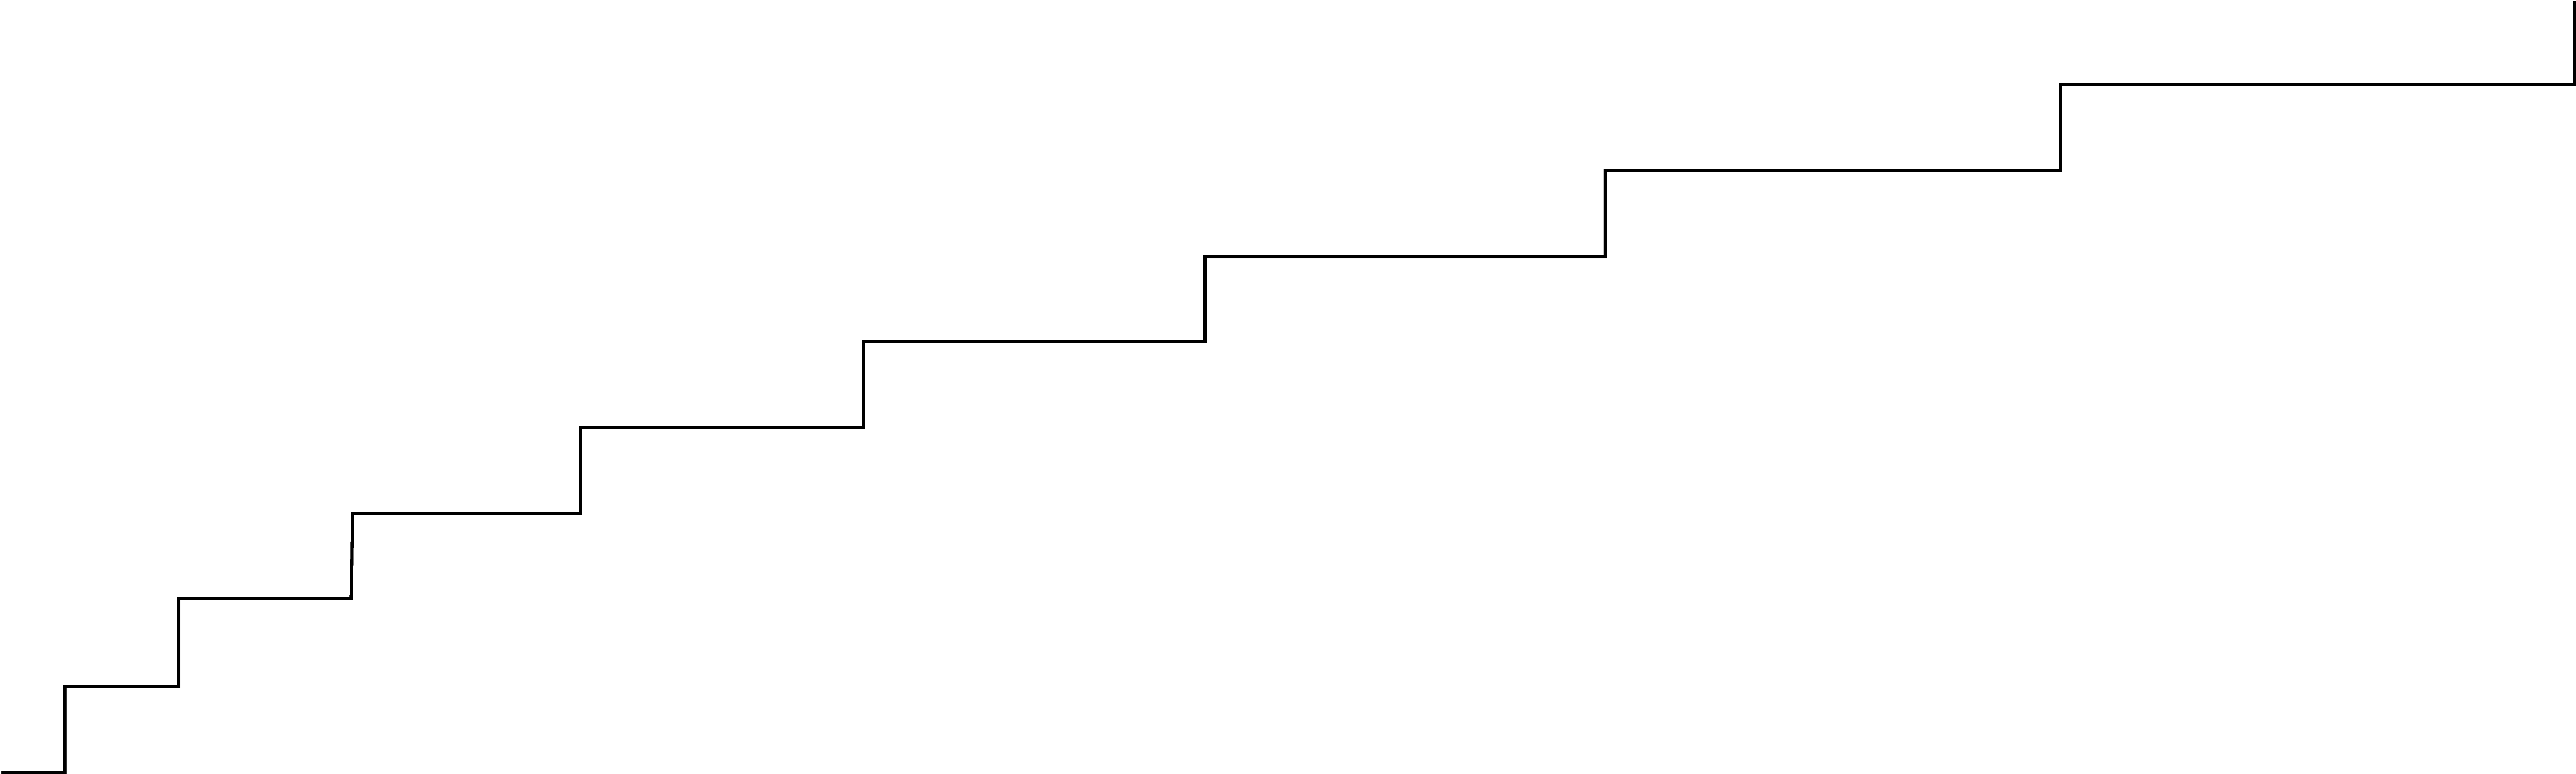
\includegraphics[scale=0.05]{Imatges/figura10-1.pdf}
\end{center}
\caption{Pica dibuixa una escala molt estranya.}
\label{fig1001}
\end{figure}

Una solució senzilla la mostrem a l'\emph{script}~\ref{scr10-1}, on la longitud de cada esglaó creix 10 píxels. Aquesta solució, però, no és satisfactòria per dues raons: Primera, heu de calcular la longitud de cada esglaó manualment. I segona, heu d'escriure molts cops una seqüència de missatges que varia molt poc a cada repetició.
\begin{script}  Pica dibuixa l'escala estranya.
\textsf{\upshape
\begin{tabbing}
\hspace{5mm} \= \kill
$|$ pica $|$\\
pica := Bot nou.\\
pica ves: 10.\\
pica giraEsquerra: 90.\\
pica ves: 5.\\
pica giraDreta: 90.\\
pica ves: 20.\\
pica giraEsquerra: 90.\\
pica ves: 5.\\
pica giraDreta: 90.\\
pica ves: 30.\\
pica giraEsquerra: 90.\\
pica ves: 5.\\
pica giraDreta: 90.\\
pica ves: 40.\\
pica giraEsquerra: 90.\\
pica ves: 5.\\
pica giraDreta: 90.\\
\dots \\
\end{tabbing}
}
\label{scr10-1}
\end{script}

Ens agradaria ser capaços d'utilitzar totes les possibilitats que ens donen les variables (per automatitzar l'increment de la mida de l'esglaó) combinades amb la potència dels bucles (de manera que no calgui repetir tant de codi). Per evitar repetir la seqüència d'enviaments de missatges podeu utilitzar el missatge \textsf{vegadesRepetir:}. I la clau de la utilització de les variables la podeu trobar en un examen atent de l'\emph{script}~\ref{scr10-1}, on podeu veure que la longitud de cada esglaó posterior al primer és la longitud de l'esglaó anterior més 10 píxels. És clar que $20=10+10$, $30=20+10$, $40=30+10$ i així successivament, com mostrem a la figura~\ref{fig1002}. \index{esglaons!mesurar per dibuixar una escala|(} \index{variables!utilitzar en dibuixar una escala}
\begin{figure}[h]
\begin{center}
\includegraphics[scale=0.1]{Imatges/figura10-2.pdf}
\end{center}
\caption{La mida d'un esglaó és la mida de l'esglaó anterior més 10 píxels.}
\label{fig1002}
\end{figure}

Utilitzem la variable \textsf{longitudEsglao} per representar la longitud d'un esglaó. Un cop \textsf{longitudEsglao} ha estat inicialitzada a la longitud del primer esglaó, l'expressió \textsf{longitudEsglao := longitudEsglao + 10} fixarà la longitud del \emph{proper} esglaó al valor del esglaó \emph{actual} incrementat en 10. El resultat és que si \textsf{longitudEsglao} s'inicialitza a 10 i dibuixem el primer esglaó, aquest esglaó tindrà òbviament mida 10. Després que l'expressió \textsf{longitudEsglao := longitudEsglao + 10} sigui executada, la propera vegada que es dibuixi un esglaó tindrà mida 20. I després que l'expressió s'executi altre cop, el proper esglaó tindrà mida 30, i així successivament.

Combinem-ho tot! Començarem amb l'\emph{script} d'una escala normal (\emph{Script}~\ref{scr10-2}). Aleshores, a l'\emph{Script}~\ref{scr10-3}, obtenim la mateixa escala però utilitzant la variable \textsf{longitudEsglao}. A l'\emph{Script}~\ref{scr10-4} afegim la línia \textsf{longitudEsglao := longitudEsglao + 10} per canviar el valor de \textsf{longitudEsglao} a cada iteració, finalment aconseguim l'escala que volem.

\begin{script}  Una escala amb esglaons normals.
\textsf{\upshape
\begin{tabbing}
\hspace{5mm} \= \kill
$|$ pica $|$\\
pica := Bot nou.\\
10 vegadesRepetir:\\
\> [ pica ves: 10.\\
\> pica giraEsquerra: 90.\\
\> pica ves: 5.\\
\> pica giraDreta: 90 ]\\
\end{tabbing}
}
\label{scr10-2}
\end{script}

\begin{script}  Una escala amb esglaons normals, utilitzant la variable \textsf{{\upshape longitudEsglao}}.
\textsf{\upshape
\begin{tabbing}
\hspace{5mm} \= \kill
$|$ pica {\bfseries longitudEsglao} $|$\\
pica := Bot nou.\\
{\bfseries longitudEsglao := 10.}\\
10 vegadesRepetir:\\
\> [ pica ves: {\bfseries longitudEsglao}.\\
\> pica giraEsquerra: 90.\\
\> pica ves: 5.\\
\> pica giraDreta: 90 ]\\
\end{tabbing}
}
\label{scr10-3}
\end{script}

\begin{script}  La solució: incrementar la variable \textsf{{\upshape longitudEsglao}} cada cop dins del bucle produeix l'escala estranya.
\textsf{\upshape
\begin{tabbing}
\hspace{5mm} \= \kill
$|$ pica {\bfseries longitudEsglao} $|$\\
pica := Bot nou.\\
{\bfseries longitudEsglao := 10.}\\
10 vegadesRepetir:\\
\> [ pica ves: {\bfseries longitudEsglao}.\\
\> pica giraEsquerra: 90.\\
\> pica ves: 5.\\
\> pica giraDreta: 90.\\
\> {\bfseries longitudEsglao := longitudEsglao + 10.} ]\\
\end{tabbing}
}
\label{scr10-4}
\end{script}

Anem a examinar més detingudament la seqüència d'expressions dins del bucle de l'\emph{Script}~\ref{scr10-4}. La primera expressió dibuixa un esglaó fent que el robot es mogui endavant una distància que ve donada pel valor de la variable \textsf{longitudEsglao} (que ha estat inicialitzada a 10 abans d'entrar dins del bucle). Aleshores el robot gira, dibuixa l'alçada de l'esglaó i gira un altre cop. Llavors el valor de la variable \textsf{longitudEsglao} s'incrementa en 10 i la repetició torna a començar, tot i que ara la variable \textsf{longitudEsglao} té un valor nou, més gran que el que tenia abans. (20 a la segona repetició). Tot aquest procés s'executa 10 vegades.

L'expressió \textsf{longitudEsglao := longitudEsglao + 10} és absolutament necessària. Sense ella, el valor de la variable mai no canviaria.\index{expressions!per dibuixar una escala}

\begin{center}
\colorbox{black}{\makebox[\textwidth]{  \color{white} {\large {\bfseries Experiment 10-1 (col·locació de l'increment dins del bucle)}}}}
\end{center}
\index{colocacio@col·locació de l'increment dins del bucle, Experiment}
\index{Experiments!colocacio@col·locació de l'increment dins del bucle}
{\small
\noindent
Intenteu canviar la darrera línia del bucle; per exemple, \textsf{longitudEsglao := longitudEsglao + 15}. Aleshores proveu de moure aquesta línia a diferents llocs del bucle. Podeu explicar què passa quan moveu la darrera línia del bucle al començament del bucle?}\\
\noindent
\rule{\textwidth}{3pt}
\vspace{1mm}

Si encara no esteu del tot segurs de què està passant a l'\emph{Script}~\ref{scr10-4}, us suggerim que penseu amb cura sobre el valor de la variable \textsf{longitudEsglao}, especialment al començament i al final del bucle. Intenteu endevinar el valor de \textsf{longitudEsglao} a cada una de les expressions del bucle durant tres iteracions. Si cal, llegiu el capítol~\ref{cap8} altre cop. \index{dibuixar!escala|)} \index{escala!dibuixar|)}\index{esglaons!mesurar per dibuixar una escala|)}


\section{Pràctiques amb repeticions i variables: laberints, espirals i altres.}
\index{bucles|seealso{bucles imbricats}}
\index{variables!combinar amb bucles|(}
\index{bucles!combinar variables amb|(}
Anem a veure com, combinant variables i repeticions, podem ajudar-vos a resoldre altres problemes.
\begin{center}
\colorbox{black}{\makebox[\textwidth]{  \color{white} {\large {\bfseries Experiment 10-2 (una altra escala estranya)}} }}
\end{center}
\index{altra escala@una altra escala estranya, Experiment}
\index{Experiments!altra escala@una altra escala estranya}
{\small
\noindent
Modifiqueu l'\emph{Script}~\ref{scr10-4} per dibuixar la figura que veieu més avall, que representa una escala en què s'incrementen tant la longitud com l'alçada de l'esglaó.}
\begin{center}
\includegraphics[scale=0.25]{Imatges/figuraE10-2.png}
\end{center}
\noindent
\rule{\textwidth}{3pt}

\begin{center}
\colorbox{black}{\makebox[\textwidth]{  \color{white} {\large {\bfseries Experiment 10-3 (un senzill laberint)}} }}
\end{center}
\index{laberint senzill@un senzill laberint, Experiment}
\index{Experiments!laberint senzill@un senzill laberint}
{\small
\noindent
Escriviu un \emph{script} que reprodueixi la figura mostrada més avall. A més, canviant l'angle que gira el robot, hauríeu de ser capaços de re-crear la figura que podeu veure al començament del capítol, així com l'espiral de la figura~\ref{fig1003}. }
\begin{center}
\includegraphics[scale=0.5]{Imatges/figuraE10-3.png}
\end{center}
\noindent
\rule{\textwidth}{3pt}

\begin{figure}[h!]
\begin{center}
\includegraphics[scale=0.1]{Imatges/figura10-3.jpg}
\end{center}
\caption{Una espiral bonica.}
\label{fig1003}
\index{espiral, dibuixar}
\end{figure}

\begin{center}
\colorbox{black}{\makebox[\textwidth]{  \color{white} {\large {\bfseries Experiment 10-4 (quadrats russos)}} }}
\end{center}
\index{quadrats russos, Experiment}
\index{Experiments!quadrats russos}
\index{midaCostat paràmetre!utilitzar a l'experiment dels quadrats russos}
{\small
\noindent
Dibuixeu els quadrats encaixats de diferentes mides com mostrem a la figura de més avall. Podríeu començar definint un bucle que dibuixi el mateix quadrat deu vegades. Aleshores introduïu una variable \textsf{longitudCostat} per representar la longitud del costat del quadrat, i finalment, feu que el costat s'incrementi a cada iteració del bucle. Com a repte addicional, podríeu provar d'escriure un nou \emph{script} que dibuixi la mateixa figura sense que el robot salti o dibuixi cap línia dos cops.}
\begin{center}
\includegraphics[scale=0.75]{Imatges/figuraE10-4.png}
\end{center}
\noindent
\rule{\textwidth}{3pt}

\begin{center}
\colorbox{black}{\makebox[\textwidth]{  \color{white} {\large {\bfseries Experiment 10-5 (un passadís llarg)}} }}
\end{center}
\index{passadís llarg@un passadís llarg, Experiment}
\index{Experiments!passadís llarg@un passadís llarg}
\index{quadrats concèntrics, dibuixar}
{\small
\noindent
Els quadrats concèntrics (que tenen el mateix centre) de diferentes mides mostrats a la figura de més avall representen un llarg passadís, que sembla fer-se més petit a mida que l'anem veient de més lluny. Altre cop, comenceu dibuixant un quadrat, però aquest cop dibuixeu-lo començant des del mig (us caldrà un missatge \textsf{salta:}), de manera que quan canvieu la mida del quadrat, el proper quadrat serà dibuixat automàticament concèntric al primer. Ara definiu el vostre quadrat dins d'un bucle, i introduïu la variable \textsf{longitudCostat} representant la longitud del costat del quadrat. Finalment, incrementeu la longitud del costat del quadrat a cada iteració.}
\begin{center}
\includegraphics[scale=0.25]{Imatges/figuraE10-5.png}
\end{center}
\noindent
\rule{\textwidth}{3pt}

\section{Alguns aspectes importants d'utilitzar variables i repeticions}
\index{bucles!combinar variables amb|)}
Ara que ja heu vist el procés complet de combinar repeticions i variables i heu experimentat una miqueta, ens agradaria emfatitzar alguns aspectes importants. L'\emph{Script}~\ref{scr10-5} mostra la típica situació de forma esquemàtica: Primer declarem una variable. Després aquesta variable és inicialitzada. Dins del bucle, la variable és utilitzada per fer alguns càlculs, i el seu valor és canviat per a la propera iteració.\index{variables!combinar amb bucles|)}
\begin{script}  Un esquema d'\emph{script} mostrant l'ús d'una variable dins d'un bucle.
\textsf{\upshape
\begin{tabbing}
\hspace{5mm} \= \hspace{70mm}\=\kill
$|$ {\bfseries longitudEsglao} pica $|$ \> \> {\itshape ``declaració de variables''}\\
\dots \\
{\bfseries longitudEsglao := 10.} \> \> {\itshape ``inicialització de la variable''}\\
\dots \\
10 vegadesRepetir:\\
\> [ pica ves: {\bfseries longitudEsglao}.\> {\itshape ``ús de  la variable''}\\
\> \dots \\
\> {\bfseries longitudEsglao := longitudEsglao + 10} ] \> {\itshape ``canvi de valor de la variable''}\\
\end{tabbing}
}
\label{scr10-5}
\end{script}

\subsection{Inicialització de variables}
\index{inicialització de variables}
\index{variables!inicialitzar}
Quan introduïu una variable en un bucle, heu de posar especial atenció al valor inicial de la variable, és a dir, al valor assignat a la variable quan és inicialitzada. Recordeu que una variable no pot ser utilitzada fins que ha estat inicialitzada. Usualment, la inicialització de les variables es fa fora del bucle, ja que d'una altra manera el valor de la variable seria reinicialitzat a cada iteració, i aquest valor no canviaria mai.

\subsection{Utilitzar i canviar el valor d'una variable}
\index{variables!utilitzar}
\index{variables!introduir en bucles}
\index{bucles!introduir variables als}
\index{variables!canviar el valor de les}
\index{valors!canviar el d'una variable}
Dins del bucle, el valor de la variable s'utilitza sovint per realitzar càlculs diversos, com calcular els valors d'altres variables o dir-li a un robot a quina distància s'ha de moure. Per tant, el valor d'una variable eventualment es canvia. A l'exemple de l'escala, l'expressió \textsf{longitudEsglao := longitudEsglao + 10} incrementa el valor de la longitud de l'esglaó basant-se en el seu valor anterior. El que és important d'entendre és que el nou valor assignat a la variable serà el seu valor a la propera volta del bucle, com veieu a la figura~\ref{fig1004}.

\begin{figure}
\begin{center}
\includegraphics[scale=0.135]{Imatges/figura10-4.pdf}
\end{center}
\caption{La longitud d'un esglaó és la longitud de l'esglaó anterior més 10 píxels. El darrer valor que una variable té dins del bucle és el valor que la variable tindrà al començament del bucle quan es repeteixi.}
\label{fig1004}
\end{figure}
\newpage

\section{Experiments avançats}

\begin{center}
\colorbox{black}{\makebox[\textwidth]{  \color{white} {\large {\bfseries Experiment 10-6 (quadrats)}} }}
\end{center}
\index{quadrats, Experiment}
\index{Experiments!quadrats}
\index{tauler, construcció de}
{\small
\noindent
Definiu un \emph{script} que dibuixi el tauler que veieu més avall. Aquest experiment és una mica més complicat que els experiments anteriors, ja que és difícil veure com dibuixar la figura amb una sola repetició. Tot i així, hi ha diverses maneres de resoldre el problema utilitzant dos bucles. Per exemple, podríeu utilitzar un bucle per dibuixar totes les línies horitzontals i un altre per dibuixar totes les línies verticals.}
\begin{center}
\includegraphics[scale=0.3]{Imatges/figuraE10-6.png}
\end{center}
\noindent
\rule{\textwidth}{3pt}

\begin{center}
\colorbox{black}{\makebox[\textwidth]{  \color{white} {\large {\bfseries Experiment 10-7 (piràmide)}} }}
\end{center}
\index{piràmide, Experiment}
\index{Experiments!piràmide}
{\small
\noindent
Escriviu un \emph{script} que dibuixi la figura que veieu més avall, representant els blocs de pedra que formen part de la piràmide esglaonada de Saqqara, que ja coneixeu de capítols anteriors. Podríeu modificar el vostre \emph{script} de l'Experiment 10-7 canviant la variable corresponent a la longitud de la línia dibuixada a cada iteració.}
\begin{center}
\includegraphics[scale=0.45]{Imatges/figuraE10-7.png}
\end{center}
\noindent
\rule{\textwidth}{3pt}
\newpage
\section{Resum}
\index{quadrats concèntrics, dibuixar|seealso{quadrats}}
\index{binaris, missatges|seealso{missatges}}
\index{unaris, missatges|seealso{missatges}}
\index{paraula-clau, missatges|seealso{missatges}}
\begin{itemize}
\item Quan s'introdueix una variable dins d'un bucle, heu d'estar segurs d'haver-la inicialitzat correctament. Recordeu que cal inicialitzar una variable abans d'utilitzar-ne el valor. Usualment, la inicialització es fa fora del bucle, ja que si no fos així el valor de la variable no canviaria amb les repeticions del bucle.
\item Recordeu que el darrer valor que rep una variable dins d'un bucle serà el valor de la variable al començament de la següent iteració del bucle.
\end{itemize}

\chapter{Compondre missatges}
\label{cap11}
\index{binaris, missatges!exemples de|(}
\index{binaris, missatges!explicació de|(}
\index{unaris, missatges!explicació de|(}
\index{paraula-clau, missatges!exemples de|(}
\index{paraula-clau, missatges!explicació de|(}
\index{missatges!components dels}
\index{missatges!tipus de|(}
Smalltalk, com tots els altres llenguatges de programació, segueix algunes regles en executar els missatges enviats als objectes. Encara no us hem explicat aquestes regles, i és possible que us hagueu preguntat quines són quan estaveu experimentant amb els \emph{scripts} dels capítols anteriors. La vostra paciència es veurà ara recompensada. Aquest capítol explica com llegir i escriure missatges formulats correctament.

Aquest capítol pot semblar una mica més difícil o abstracte que els capítols anteriors. Tot i així, hem procurat presentar tan clarament com hem sabut les senzilles regles que governen l'escriptura de missatges. Entendre aquests detalls no és tan divertit com jugar amb els robots, però és el preu que heu de pagar si voleu ser capaços d'escriure programes més complicats. Les bones notícies són que Smalltalk no és un llenguatge complex: Hi ha només cinc regles que heu d'entendre. Si encara dubteu, podeu saltar-vos aquest capítol en una primera lectura i tornar-hi quan tingueu algun dubte sobre l'estructura dels vostres programes.

Tal com vam explicar al capítol~\ref{cap2}, un missatge està compost d'un \emph{selector de missatge} i els \emph{arguments del missatge}, si n'hi ha. Un missatge és enviat a un \emph{receptor del missatge}. La combinació del missatge i el receptor s'anomena un \emph{enviament de missatge}.

Quan escriviu una \emph{expressió} complexa, com \textsf{pica ves: 100 + 20}, aquesta conté dos enviaments de missatge, amb els selectors \textsf{ves:} i \textsf{$+$}, i heu de conèixer en quin ordre són executats els missatges si voleu entendre el resultat de l'expressió. A Smalltalk, l'ordre en què els missatges s'executen ve determinat pel \emph{tipus} de l'enviament de missatge. N'hi ha tres tipus: \emph{unaris}, \emph{binaris} i \emph{paraula-clau}. Els missatges unaris sempre s'envien els primers, seguits dels missatges binaris i finalment els missatges de paraula-clau. Els missatges posats entre parèntesis s'executen abans que qualsevol altre tipus de missatge. Això vol dir que podeu canviar l'ordre en què els enviaments de missatges són executats mitjançant la col·locació de parèntesis. Aquestes regles són en gran part responsables que el codi Smalltalk sigui fàcil de llegir. I aviat descobrireu que la majoria de les vegades ni tan sols us caldrà pensar-hi. Tot i així, heu de conèixer aquestes regles, ja que pot ser que en alguna ocasió sí que us calgui saber-les aplicar.\index{expressions!components de}

Tots els exemples que apareixen en aquest capítol són codi executable, tal com es mostra en el text. No dubteu a provar-los i entendre com funcionen. Començarem ensenyant-vos la manera d'identificar els diferents tipus de missatges, i després presentarem alguns exemples de cada tipus. Finalment, introduirem les regles per a la composició de missatges.

\section{Els tres tipus de missatges}

Smalltalk defineix un petit nombre de regles senzilles per determinar l'ordre en què s'executen els missatges. Aquestes regles, que presentarem en detall més tard, es basen en la diferenciació dels missatges en tres tipus:

\begin{itemize}
\item \emph{Missatges unaris} són missatge sense arguments. Són enviats a un objecte (el receptor del missatge) sense cap altra informació. Per exemple, a l'expressió \textsf{pica color}, el missatge \textsf{color} és un missatge unari. No envia cap informació addicional; això vol dir que no hi ha cap argument. Aquests missatges s'anomenen ``unaris'' del Llatí \emph{unum}, que significa ``un'', ja que un enviament de missatge amb un missatge unari involucra \emph{només un objecte}, el receptor del missatge.
\item \emph{Missatges binaris}, són missatges que involucren \emph{dos objectes}: el receptor del missatge i l'únic argument del selector del missatge (la paraula ``binari'' ve del Llatí \emph{bis}, que significa ``dues vegades''). Els missatges binaris usualment s'utilitzen en expressions matemàtiques. Per exemple, a l'enviament de missatge \textsf{10 + 20}, el missatge consta del selector de missatge \textsf{$+$} juntament amb el seu únic argument \textsf{20}. El missatge \textsf{+ 20} és enviat a l'objecte \textsf{10}, que és el receptor del missatge. \index{objectes!relació amb missatges binaris}
\item \emph{Missatges de paraula-clau}, són missatges el selector dels quals conté almenys una paraula clau amb un caràcter ``dos punts'' (:) al seu nom i que té un o més arguments. Per exemple, al missatge \textsf{pica ves: 100}, la paraula clau \textsf{ves:} conté el caràcter ``dos punts'' (:), hi ha un argument, \textsf{100}, i per tant hi ha dos objectes involucrats en l'enviament de missatge: el receptor del missatge \textsf{pica} i l'argument \textsf{100}.
\end{itemize}

\newpage

\noindent
\rule{\textwidth}{2pt}
\noindent
\textbf{Nota} No us confongueu per la nomenclatura dels missatges unaris i binaris. La idea d' ``un'' a la paraula \emph{unari} i la idea de ``dos'' a la paraula \emph{binari} es refereixen al nombre d'objectes involucrats en l'enviament del missatge, no al nombre d'arguments. Així, un missatge unari no té cap argument, però hi participa un objecte, el receptor del missatge. Un missatge binari té només un argument, i per tant un enviament de missatge d'un missatge binari implica dos objectes: l'argument del selector del missatge i el receptor del missatge.\\
\noindent
\rule{\textwidth}{2pt}

\section{Identificar missatges}
\index{binaris, missatges!exemples de|)}
\index{binaris, missatges!explicació de|)}
\index{unaris, missatges!explicació de|)}
\index{paraula-clau, missatges!exemples de|)}
\index{paraula-clau, missatges!explicació de|)}
\index{missatges!identificar|(}
\index{missatges!tipus de|)}
Per poder entendre l'estructura d'una expressió, el primer que us cal fer és identificar els missatges i els seus receptors. Per tal de fer això, us suggerim que utilitzeu una notació gràfica com la que veieu a la figura~\ref{fig1101}. En totes les figures d'aquest capítol, els receptors de missatge estan \emph{subratllats}, cada missatge està envoltat d'una \emph{el·lipse}, i els missatges que constitueixen l'expressió estan \emph{numerats} en l'ordre en què s'executaran. Quan hi ha més d'una el·lipse, la primera el·lipse a executar es dibuixa amb una línia interrompuda de manera que es pugui veure de seguida on començar.\index{elipses@el·lipses!al voltant dels missatges, significat de}

La figura~\ref{fig1101} mostra que l'expressió \textsf{pica color: Color groc} conté l'expressió \textsf{Color groc}. Per tant hi ha dues el·lipses, una per a l'expressió completa \textsf{pica color: Color groc} i una altra per a la subexpressió \textsf{Color groc}. Aprendreu una mica més endavant que l'expressió \textsf{Color groc} s'executa primer, de manera que l'el·lipse està dibuixada amb línia interrompuda i s'ha numerat amb el nombre 1. Fixeu-vos que cada missatge té un receptor. El robot \textsf{pica} rep el missatge \textsf{color: \dots}, i \textsf{Color} rep el missatge \textsf{groc}. Per tant, aquests dos receptors de missatge estan subratllats (els tres punts al missatge \textsf{color: \dots} indiquen l'argument del selector de missatge \textsf{color:}, que serà el resultat de l'enviament de missatge \textsf{Color groc}). \index{subratllats, receptors de missatge; significat de|(}
\begin{figure}[h]
\begin{center}
\includegraphics[scale=0.25]{Imatges/figura11-1.pdf}
\end{center}
\caption{L'expressió \textsf{\upshape pica color: Color groc} conté la subexpressió \textsf{\upshape Color groc}. El missatge \textsf{\upshape groc} és enviat a \textsf{\upshape Color}, i després el missatge \textsf{\upshape color: \dots} és enviat a \textsf{\upshape pica}.}
\label{fig1101}
\index{unaris, missatges!exemples de}
\end{figure}

Tal com hem dit, cada missatge és enviat a un objecte anomenat el receptor del missatge. Un receptor no ha de ser un robot. Pot ser qualsevol cosa, des d'un nombre a una finestra. Un receptor de missatge pot aparèixer explícitament com a primer element d'una expressió, com \textsf{pica} a l'expressió \textsf{pica ves: 100} o \textsf{Color} a l'expressió \textsf{Color blau}. Un receptor, però, també pot ser el resultat d'altres enviaments de missatges. Per exemple, al missatge \textsf{Bot nou ves: 100}, el receptor del missatge \textsf{ves: 100} és l'objecte resultant del retorn de l'enviament de missatge \textsf{Bot nou}. Tot i així, un missatge sempre és enviat a algun objecte, i aquest objecte és anomenat receptor del missatge.\index{arguments!indicar pels receptors dels missatges} \index{missatge, enviaments de!efecte de} \index{receptors!explicació de} \index{indicar els arguments per a}

\noindent
\rule{\textwidth}{2pt}
\noindent
\textbf{Important!} En un \emph{enviament de missatge}, un \emph{missatge} és sempre enviat a un \emph{objecte}, anomenat el \emph{receptor del missatge}, que pot ser explícit o el resultat d'altres enviaments de missatge.

\noindent
\rule{\textwidth}{2pt}
\vspace{3mm}

La taula~\ref{tab1101} mostra alguns enviaments de missatge; us suggerim que en cada cas identifiqueu el tipus de missatge i dibuixeu la representació gràfica de l'expressió.
\begin{table}[h]
\caption{Alguns exemples d'enviaments de missatge, simples i compostos.}
\label{tab1101}
\begin{center}
{\small \begin{tabular}{p{40mm}p{40mm}p{60mm}}
\hline
\textbf{Expressió} & \textbf{Tipus} & \textbf{Acció}\\
\hline
\textsf{pica ves: 100} & paraula-clau & El robot receptor es mou endavant 100 píxels.\\
\textsf{100 + 20} & binari & El nombre \textsf{100} rep el missatge \textsf{$+$} amb el nombre \textsf{20} com a argument.\\
\textsf{pica est} & unari & El robot receptor \textsf{pica} apunta a l'\textsf{est}\\
\textsf{pica color: Color groc} & paraula-clau, unari & El robot receptor \textsf{pica} canvia els seu color pel color groc\\
\textsf{pica ves: 100 + 20} & paraula-clau, binari & El robot receptor es mou endavant 120 píxels.\\
\textsf{Bot nou ves: 100} & unari, paraula-clau & El missatge \textsf{nou} és enviat a la classe \textsf{Bot}, que retorna un robot nou al qual el missatge \textsf{ves: 100} és enviat, fent que el robot es mogui endavant 100 píxels.\\
\hline
\end{tabular}}
\end{center}
\end{table}

A partir de la taula~\ref{tab1101} hauríeu de parar atenció a les següents observacions:
\begin{itemize}
\item Alguns missatges tenen arguments, altres missatges no. El missatge \textsf{est}, sent unari, no té cap argument, mentre que \textsf{ves: 100} i \textsf{+ 20} tenen cadascun un argument, el nombre \textsf{100} i el nombre \textsf{20} respectivament.
\item S'envien diferents missatges a diversos objectes. A l'expressió \textsf{pica est}, el missatge \textsf{est} és enviat a un robot, i a \textsf{100 + 20}, el missatge \textsf{+ 20} és enviat al nombre \textsf{100}.
\item Hi ha missatges simples i missatges compostos. Per exemple, \textsf{Color groc} i \textsf{100 + 20} són simples: Un missatge és enviat a un objecte. Per altra part, l'expressió \textsf{pica ves: 100 + 20} conté dos missatges: \textsf{+ 20} és enviat a \textsf{100}, i després \textsf{ves: \dots} és enviat a \textsf{pica}, on \textsf{\dots} representa el resultat de l'execució de l'enviament de missatge \textsf{100 + 20}. 
\item El receptor de missatge pot ser el resultat d'una expressió que retorna un objecte. A l'expressió \textsf{Bot nou ves: 100}, el missatge \textsf{ves: 100} és enviat a l'objecte (un robot) que resulta de l'avaluació de l'expressió \textsf{Bot nou}.
\end{itemize}

\section{Els tres tipus de missatges en detall}
\index{missatges!identificar|)}
\index{subratllats, receptors de missatge; significat de|)}
Ara que ja sou capaços d'identificar els receptors de missatge i els tres tipus de missatges, examinem en detall els diferents tipus de missatges.

\subsection{Missatges unaris}

Entre els usos habituals dels missatges unaris hi ha l'obtenció d'un valor a partir d'un objecte, com la mida del llapis d'un robot (\textsf{pica midaLlapis}); obtenir un objecte a partir d'una classe (\textsf{Color groc}); i ordenar al receptor la realització d'alguna acció (\textsf{pica tornarInvisible}). Recordeu que un missatge unari no té arguments: és enviat al receptor sense cap més informació. Així, l'únic objecte implicat en un enviament de missatge unari és el receptor del missatge. Enviaments de missatge unaris són de la forma \textsf{{\itshape receptor nomMissatge}}. L'\emph{Script}~\ref{scr11-1} presenta alguns exemples de missatges unaris, mostrats en negreta.
\begin{script}  Exemples de missatges unaris.
\textsf{\upshape
\begin{tabbing}
\hspace{5mm} \= \kill
$|$ pica $|$\\
pica := Bot {\bfseries nou}.\\
pica {\bfseries color}.\\
pica {\bfseries midaLlapis}.\\
pica {\bfseries est}.\\
Color {\bfseries groc}.\\
125 {\bfseries factorial}.\\
\end{tabbing}
}
\label{scr11-1}
\index{unaris, missatges!exemples de}
\end{script}
\noindent
\rule{\textwidth}{2pt}
\noindent
\textbf{Important!} Els missatges unaris són missatges que no tenen cap argument. Un enviament de missatge unari té la forma \textsf{{\itshape receptor nomMissatge}}.

\noindent
\rule{\textwidth}{2pt}

\subsection{Missatges binaris}
\index{binaris, missatges!exemples de}
\index{objectes!en missatges binaris}
Els missatges binaris són missatges que involucren dos objectes: el receptor i un únic argument. Tots els selectors de missatges dels missatges binaris consisteixen en un o dos caràcters de la llista següent: \textsf{$+$}, \textsf{$*$}, \textsf{$/$}, \textsf{$|$}, \textsf{\&}, \textsf{$=$}, \textsf{$>$}, \textsf{$<$}, \textsf{$\sim$}, \textsf{@}. Per tant, \textsf{$+$},  \textsf{$=$} i  \textsf{$*$} són selectors de missatge, però també ho és  \textsf{$=>$}, que està compost de dos símbols.

La taula~\ref{tab1102} mostra alguns exemples d'enviaments de missatge binari i el seu significat. Ara mateix, no entrarem en els detalls d'aquests exemples, no us amoïneu si no esteu completament segurs del que fan tots i cadascun d'aquests selectors de missatge. Proveu, però, d'executar les expressions i altres de similars.

\begin{table}[h]
\caption{Exemples de missatges binaris numèrics.}
\label{tab1102}
\begin{center}
{\small \begin{tabular}{p{25mm}p{40mm}p{75mm}}
\hline
\textbf{Expressió} & \textbf{Valor Retornat} & \textbf{Acció}\\
\hline
\textsf{1 + 2.5} & \textsf{3.5} & 
Suma de dos nombres\\
\textsf{3.4 \textsf{$*$} 5} & \textsf{17.0} & 
Producte de dos nombres\\
\textsf{8 / 2} & \textsf{4} & 
Divisió de dos nombres\\
\textsf{10 - 8.3} & \textsf{1.7} & 
Resta de dos nombres\\
\textsf{12 $=$ 11} & \textsf{false} & 
Test d'igualtat entre nombres\\
\textsf{12 $\sim=$ 11} & \textsf{true} & 
Test de desigualtat entre nombres\\
\textsf{12 $>$ 9} & \textsf{true} & 
És el receptor més gran que l'argument?\\
\textsf{12 $>=$ 10} & \textsf{true} & 
És el receptor més gran o igual que l'argument?\\
\textsf{12 $<$ 10} & \textsf{false} & 
És el receptor més petit que l'argument?\\
\textsf{100@10} & \textsf{100@10} & 
Crea un punt amb coordenades (100,10)\\
\hline
\end{tabular}}
\end{center}
\end{table}

\noindent
\rule{\textwidth}{2pt}
\noindent
\textbf{Important!} Els enviaments de missatge binari involucren dos objectes: el receptor i un únic argument. El selector de missatge d'un missatge binari està compost d'un o dos caràcters de la llista següent:  \textsf{$+$}, \textsf{$*$}, \textsf{$/$}, \textsf{$|$}, \textsf{\&}, \textsf{$=$}, \textsf{$>$}, \textsf{$<$}, \textsf{$\sim$}, \textsf{@}. Els enviaments de missatge binari tenen la forma \textsf{{\itshape receptor nomMissatge argument}}.

\noindent
\rule{\textwidth}{2pt}

\subsection{Missatges de paraula-clau}
\index{paraula-clau, missatges!exemples de}
Els missatges de paraula-clau són missatges que prenen com a mínim un argument i contenen com a mínim un caràcter ``dos punts'' (:). Fixeu-vos que els dos punts formen part del selector de missatge. Per tant, \textsf{ves:}, no \textsf{ves}, és el nom d'un missatge de paraula-clau. L'\emph{Script}~\ref{scr11-2} presenta alguns exemples de missatges de paraula-clau, mostrats en negreta.
\begin{script}  Exemples de missatges de paraula-clau.
\textsf{\upshape
\begin{tabbing}
\hspace{5mm} \= \kill
$|$ pica $|$\\
pica := Bot nou.\\
pica {\bfseries ves:} 100.\\
pica {\bfseries midaLlapis:} 5.\\
pica {\bfseries color:} Color groc.\\
pica {\bfseries gira:} 90.\\
\end{tabbing}
}
\label{scr11-2}
\end{script}

Ja hem dit que els missatges de paraula-clau tenen com a mínim un argument, però encara no hem vist cap exemple d'un missatge amb múltiples arguments. L'enviament de missatge\footnote{\emph{Nota del Traductor:} Altre cop, aquest missatge pertany a Smalltalk més que a l'entorn \textsf{BotInc}, per tant no l'hem traduït.} \textsf{{\itshape unNumero} between: {\itshape fitaInferior} and: {\itshape fitaSuperior}} mira si el nombre \textsf{{\itshape unNumero}} és a l'interval representat pels dos nombres \textsf{{\itshape fitaInferior}}  i \textsf{{\itshape fitaSuperior}}. El missatge necessita dos arguments, els dos extrems de l'interval. En mostrem un exemple a la taula~\ref{tab1103}. Fixeu-vos que el selector de missatge és \textsf{between:and:}. Està compost de les dues paraules  \textsf{between:} i \textsf{and:}.\index{arguments!en missatges de paraula-clau}
\begin{table}[h]
\caption{Missatges de paraula-clau que necessiten més d'un argument.}
\label{tab1103}
\begin{center}
{\small \begin{tabular}{p{35mm}p{20mm}p{35mm}p{40mm}}
\hline
\textbf{Expressió} & \textbf{Arguments} & \textbf{Valor Retornat} & \textbf{Acció}\\
\hline
\textsf{5 {\bfseries between:} 2 {\bfseries and:} 10} & \textsf{2, 10} & \textsf{true} &
Està 5 entre 2 i 10?\\
\textsf{Color {\bfseries r:} 0 {\bfseries g:} 1 {\bfseries b:} 0} & \textsf{0, 1, 0} & un objecte-color verd &
Crea un color amb els valors donats de vermell, verd i blau.\\
\hline
\end{tabular}}
\end{center}
\end{table}

\noindent
\rule{\textwidth}{2pt}
\noindent
\textbf{Important!} Els missatges de paraula-clau necessiten com a mínim un argument, i el seu selector de missatge conté com a mínim un caràcter ``dos punts'' (:). Un enviament de missatge de paraula-clau amb dos arguments pren la forma \textsf{{\itshape receptor primeraParaulaNomMissatge: primerArgument segonaParaulaNomMissatge: segonArgument}}.

\noindent
\rule{\textwidth}{2pt}

\section{Ordre d'execució}
\index{Regla 1 de l'ordre d'execució!explicació de}
\index{Regla 2 de l'ordre d'execució!explicació de}
\index{Regla 3 de l'ordre d'execució!explicació de}
\index{() (parèntesi)!inclosos per alterar l'ordre d'execució|(}
\index{parèntesi (())!inclosos per alterar l'ordre d'execució|(}
\index{ordre d'execució!panorama general|(}
\index{unaris, missatges!ordre d'execució}
Ja sabeu que hi ha tres tipus de missatges: unaris, binaris i de paraula-clau. Ara us explicarem, com vam prometre, la manera de determinar l'ordre en què són executats els missatges. L'ordre d'execució dels missatges ve donat pel tipus de missatge, tal com està descrit en les tres regles següents: \index{ordre d'execució!Regla 1}\index{ordre d'execució!Regla 2}\index{ordre d'execució!Regla 3}
\begin{itemize}
\item[] \textbf{Regla 1:} Els enviaments de missatge unari s'executen primer, després els enviaments de missatge binari i finalment els enviaments de missatge de paraula-clau.
\item[] \textbf{Regla 2:} Tal com passa amb les expressions matemàtiques, la prioritat d'execució dels missatges pot ser invalidada mitjançant la col·locació de parèntesis: els enviaments de missatge entre parèntesis s'executen abans que qualsevol altre tipus d'enviament de missatge.
\item[] \textbf{Regla 3:} Els enviaments de missatge del mateix tipus s'executen d'esquerra a dreta.
\end{itemize}

Aquestes regles poden semblar complicades, però són força naturals, i un cop us hi acostumeu, pràcticament no hi haureu de tornar a pensar. En particular, la tercera regla senzillament diu que els missatges del mateix tipus s'executen en l'ordre en el qual són llegits.

Si mai teniu dubtes, i voleu assegurar-vos que els vostres missatges s'executen en l'ordre que cal, sempre podeu afegir parèntesis extra, com veieu a la figura~\ref{fig1102}. A la figura, s'analitza l'expressió \textsf{pica color: Color groc}. El selector de missatge \textsf{groc} és un missatge unari, mentre que el selector de missatge \textsf{color:} és un missatge de paraula-clau. Per tant, l'expressió \textsf{Color groc} s'executa primer. Si no esteu convençuts de l'ordre d'execució, podeu posar parèntesis al voltant de \textsf{Color groc} per assegurar-vos que aquesta expressió serà executada primer. És a dir, \textsf{pica color: Color groc} i  \textsf{pica color: (Color groc)} tenen exactament el mateix efecte. La resta d'aquesta secció il·lustra cada un d'aquests aspectes.
\begin{figure}[h]
\begin{center}
\includegraphics[scale=0.2]{Imatges/figura11-2.pdf}
\end{center}
\caption{Els missatges unaris s'executen primer, de manera que \textsf{\upshape Color groc} és la primera expressió a executar-se. Aquesta execució retorna un objecte color, que es passa com a argument del missatge \textsf{\upshape color: \dots}, que és enviat a \textsf{\upshape pica}.}
\label{fig1102}
\end{figure}
\index{() (parèntesi)!inclosos per alterar l'ordre d'execució|)}
\index{parèntesi (())!inclosos per alterar l'ordre d'execució|)}
\subsection{Regla 1: Unari $>$ Binari $>$ Paraula-Clau}
\index{Unari $>$ Binari $>$ Paraula-clau ordre d'execució, exemples de|(}
\index{Regla 1 de l'ordre d'execució!Unari $>$ Binari $>$ Paraula-clau|(}
\index{missatges compostos!representar|(}
\index{ordre d'execució!panorama general|)}
\index{ordre d'execució!Regla 1|(}
Els enviaments de missatge unari s'executen primer, després els enviaments de missatge binari i finalment els enviaments de missatge de paraula-clau. En l'argot de la programació diem que els missatges unaris tenen \emph{precedència} sobre els missatges binaris, i que els missatges binaris tenen precedència sobre els missatges de paraula-clau.

\noindent
\rule{\textwidth}{2pt}
\noindent
\textbf{Important!} Regla 1: Els enviaments de missatge unari s'executen abans que els enviaments de missatge binari, que s'executen abans que els enviaments de missatge de paraula-clau.

\noindent
\rule{\textwidth}{2pt}

\subsubsection*{Exemple 1}

A l'enviament de missatge \textsf{pica color: Color groc}, hi ha un missatge unari, \textsf{groc}, enviat a la classe \textsf{Color}, i hi ha un missatge de paraula-clau, \textsf{color: \dots}, enviat al robot \textsf{pica}. Els enviaments de missatge unari s'executen primer, de manera que el primer enviament de missatge per executar és \textsf{Color groc}. Aquesta execució retorna un objecte color, representat com a \textsf{{\itshape unColor}} (ja que ens cal un nom), que es passa a \textsf{pica} com a argument del missatge \textsf{color: {\itshape unColor}}. La figura~\ref{fig1102} mostra gràficament l'ordre en què són executats els missatges.

Per ajudar-vos a entendre-ho millor, voldríem proposar una representació textual de l'execució pas a pas dels enviaments de missatge compostos.
A Pas-a-pas~\ref{ss11-1}, l'enviament de missatge per ser executat pas a pas és \textsf{pica color: Color groc}. La primera línia mostra l'enviament de missatge complet en negreta. \index{pica color: Color groc, descomposició de l'execució de}
\newtheorem{pas-a-pas}{Pas-a-pas}[chapter]
\begin{pas-a-pas} Descomposició de l'execució de \textsf{{\upshape pica color: Color groc}}
\noindent
\textsf{\upshape
\begin{tabbing}
\hspace{7mm} \= {\bfseries pica color:} \=  {\bfseries Color groc} \hspace{25mm} \= \\
(1) \> \> Color groc \> {\itshape ``unari''}\\
\> \> {\itshape -retorna$>$ unColor}\\
(2)\> pica color: {\itshape unColor} \> \> {\itshape ``paraula-clau''}\\
\end{tabbing}
}
\label{ss11-1}
\end{pas-a-pas}

Les línies de codi representen els diferents passos de l'execució enumerats en l'ordre que succeeixen. Així, \textsf{Color groc} és la primera expressió a ser executada. Fixeu-vos que les expressions han estat sagnades per alinear-se amb les seves expressions equivalents a l'enviament de missatge que hi ha a dalt de tot.

Quan l'execució d'un enviament de missatge retorna un resultat que s'utilitza en les següents execucions, la línia que segueix l'expressió executada mostra ``\textsf{{\itshape -retorna$>$}}'' seguit del resultat. Aquí l'expressió \textsf{Color groc} retorna un objecte color que hem anomenat \textsf{{\itshape unColor}} de manera que podem referir-nos-en més endavant. La segona expressió executada és \textsf{pica color: {\itshape unColor}}, on, com acabem d'explicar, \textsf{{\itshape unColor}} és el resultat obtingut del pas d'execució previ. Per emfatitzar això, el valor retornat és escrit en itàlica. El tipus del missatge que s'està executant s'escriu com a comentari dins de cometes, per deixar-ho més clar. Per exemple, es diu explícitament que \textsf{Color groc} és un missatge unari.

\subsubsection*{Exemple 2}
\index{missatges compostos!representar|)}
L'enviament de missatge \textsf{pica ves: 100 + 20}, conté el selector de missatge binari \textsf{$+$} i el selector de missatge de paraula-clau \textsf{ves:}.
Els missatges binaris s'executen abans que els missatges de paraula-clau, per tant \textsf{100 + 20} s'executa primer: El missatge \textsf{+ 20} és enviat a l'objecte \textsf{100}, que retorna el nombre \textsf{120}. Després el missatge \textsf{pica ves: 120} s'executa amb 120 com a argument. Pas-a-pas~\ref{ss11-2} mostra com s'executa l'expressió.\index{pica ves: 100 + 20 expressió, descomposició de}
\begin{pas-a-pas} Descomposició de l'expressió \textsf{{\upshape pica ves: 100 + 20}}
\newline
\newline
\noindent
\includegraphics[scale=0.3]{Imatges/figuraSS11-2.pdf}
\noindent
\textsf{\upshape
\begin{tabbing}
\hspace{7mm} \= {\bfseries pica ves:} \= {\bfseries 100 + 20} \= \hspace{30mm} \= \\
(1) \> \> 100 + 20 \> {\itshape ``binari''}\\
\> \> {\itshape -retorna$>$ 120}\\
(2)\> pica ves: 120 \> \> {\itshape ``paraula-clau''}\\
\end{tabbing}
}
\label{ss11-2}
\end{pas-a-pas}

\subsubsection*{Exemple 3}

El missatge \textsf{pica midaLlapis: pica midaLlapis + 2} conté el missatge unari \textsf{midaLlapis}, el missatge binari amb selector \textsf{$+$}, i el missatge de paraula-clau amb selector \textsf{midaLlapis:}. Pas-a-pas~\ref{ss11-3} il·lustra la descomposició de l'execució del missatge. L'enviament de missatge unari \textsf{pica midaLlapis} s'executa primer (pas 1). Aquest missatge retorna un nombre, que anomenarem \textsf{{\itshape unNumero}}, representant la mida de llapis actual  del receptor. Després s'executa l'enviament de missatge binari \textsf{{\itshape unNumero} + 2} (pas 2). El nombre \textsf{{\itshape unNumero}} és el receptor del missatge \textsf{+ 2}, que retorna un altre nombre, la suma, que anomenem \textsf{{\itshape unAltreNumero}}. Finalment, el missatge de paraula-clau \textsf{midaLlapis: {\itshape unAltreNumero}} és enviat a \textsf{pica}, que fa que \textsf{{\itshape unAltreNumero}} sigui la seva mida de llapis actual.

Tot plegat, l'expressió sencera incrementa la mida del llapis del receptor en dos píxels. Ho fa demanant primer la mida del seu llapis a \textsf{pica}, afegint dos a aquest nombre (\textsf{{\itshape unNumero} + 2}), i després dient-li a \textsf{pica} que canviï la mida del seu llapis pel nou nombre (\textsf{pica midaLlapis: {\itshape unAltreNumero}}). Fixeu-vos que \textsf{midaLlapis} i \textsf{midaLlapis:} són dos selectors de missatge diferents! El primer és unari i \emph{demana} al receptor la mida del seu llapis, i el segon és de paraula-clau i \emph{ordena} al receptor que canviï la seva mida de llapis pel valor de l'argument.\index{pica midaLlapis: pica midaLlapis + 2 expressió, descomposició de}

\begin{pas-a-pas} Descomposició de l'expressió \textsf{{\upshape pica midaLlapis: pica midaLlapis + 2}}
\newline
\newline
\noindent
\includegraphics[scale=0.2]{Imatges/figuraSS11-3.pdf}
\noindent
\textsf{\upshape
\begin{tabbing}
\hspace{7mm} \= {\bfseries pica midaLlapis:} \= {\bfseries pica midaLlapis + 2} \hspace{20mm} \= \\
(1) \> \> pica midaLlapis \> {\itshape ``unari''}\\
\> \> {\itshape -retorna$>$ unNumero}\\
(2) \> \> {\itshape unNumero} + 2 \> {\itshape ``binari''}\\
\> \> {\itshape -retorna$>$ unAltreNumero}\\
(3) \> pica midaLlapis: {\itshape unAltreNumero} \> \> {\itshape ``paraula-clau''}\\
\end{tabbing}
}
\label{ss11-3}
\end{pas-a-pas}

\subsubsection*{Exemple 4}

Com a exercici, us deixarem descompondre l'execució del missatge \textsf{Bot nou ves: 100 + 20}, que està compost d'un missatge unari, un missatge de paraula-clau i un missatge binari (figura~\ref{fig1103}).\index{missatge Bot nou ves: 100 + 20, descomposició}
\begin{figure}[h]
\begin{center}
\includegraphics[scale=0.275]{Imatges/figura11-3.pdf}
\end{center}
\caption{Descompondre  \textsf{\upshape Bot nou ves: 100 + 20} }
\label{fig1103}
\end{figure}

\subsection{Regla 2: Primer els parèntesis}
\index{Regla 1 de l'ordre d'execució!Unari $>$ Binari $>$ Paraula-clau|)}
\index{Unari $>$ Binari $>$ Paraula-clau ordre d'execució, exemples de|)}
\index{Regla 2 de l'ordre d'execució!primer els parèntesis|(}
\index{ordre d'execució!Regla 1|)}
\index{ordre d'execució!Regla 2|(}
\index{Primer els Parèntesis, ordre d'execució; exemples de|(}
L'ordenació per defecte de l'execució de missatges pot no ser l'adequada pel que voleu fer amb una expressió, per tant hauríeu de poder canviar aquesta ordenació. Per poder fer això, Smalltalk us dóna la possibilitat d'utilitzar parèntesis ( i ). Igual que en matemàtiques, les expressions entre parèntesis tenen la precedència màxima, i s'executen abans que qualsevol altra cosa.

Recordeu que si trobeu les regles per a l'ordre d'execució complicades o si senzillament voleu deixar més clara l'estructura d'una expressió, utilitzeu parèntesis per assegurar que l'execució dels missatges es fa en l'ordre que vosaltres voleu. La figura~\ref{fig1104} mostra algunes de les expressions que hem vist anteriorment juntament amb les expressions equivalents utilitzant parèntesis.
\begin{figure}[h]
\begin{center}
\includegraphics[scale=0.15]{Imatges/figura11-4.pdf}
\end{center}
\caption{Missatges equivalents utilitzant parèntesis.}
\label{fig1104}
\end{figure}

\noindent
\rule{\textwidth}{2pt}
\noindent
\textbf{Important!} Regla 2: Igual que en matemàtiques, els missatges entre parèntesis s'executen abans que qualsevol altre missatge. Tenen la \emph{prioritat} més alta. \index{compostes, expressions, descomponent considerant els parèntesis}

\noindent
\rule{\textwidth}{2pt}

\subsubsection*{Exemple 5}
\index{65"@325 extent: 134"@100 missatge, descompondre}
El missatge\footnote{\emph{Nota del Traductor:} Els punts de la forma \textsf{a@b} són propis de l'entorn general Squeak, per tant els seus missatges no han estat traduïts, per exemple \textsf{extent:} que retorna un rectangle. Amb els rectangles passa el mateix, per tant els missatges corresponents tampoc no han estat traduïts, per exemple, \textsf{center}.} \textsf{(65@ 325 extent: 134@100) center} retorna el centre d'un rectangle amb \textsf{(65,325)} com a cantonada superior esquerra, l'amplada del qual és 134 píxels i l'altura és 100 píxels. 
Pas-a-pas~\ref{ss11-4} ens mostra com es descompon i executa el missatge. Primer, el missatge dins dels parèntesis és executat. És una expressió composta consistent en tres enviaments de missatge: dos enviaments de missatge binari, \textsf{65 @ 325} i \textsf{134 @ 100}, que s'executen primer i retornen punts; i el missatge de paraula-clau \textsf{extent: \dots}, que és enviat al punt \textsf{(65,325)} i que retorna un rectangle amb la cantonada superior esquerra, l'amplada i l'altura que ja hem dit. Finalment, el missatge unari \textsf{center} és enviat a aquest rectangle, i un punt, el centre del rectangle, és retornat. Provar d'avaluar el missatge sense parèntesis donaria un error, ja que en aquest cas, el missatge unari \textsf{center} s'hauria d'executar primer enviant-lo a l'objecte \textsf{100}, que, com és un nombre, no entén el missatge \textsf{center}.\index{Primer els Parèntesis, ordre d'execució; exemples de|)}
\begin{pas-a-pas} Descomposició d'una expressió composta amb parèntesis prioritaris.
\noindent
\textsf{\upshape
\begin{tabbing}
\hspace{7mm} \= {\bfseries (65 @ 325 extent:} \=  {\bfseries 134 @ 100) center} \hspace{10mm} \= \\
(1) \> 65 @ 325 \> \> {\itshape ``binari''}\\
\> {\itshape -retorna$>$ unPunt}\\
(2) \> \> 134 @ 100 \> {\itshape ``binari''}\\
\> \> {\itshape -retorna$>$ unAltrePunt}\\
(3) \> {\itshape unPunt} extent: {\itshape unAltrePunt} \> \> {\itshape ``paraula-clau''}\\
\> {\itshape -retorna$>$ unRectangle}\\
(4) \> {\itshape unRectangle} center \> \> {\itshape ``unari''}\\
\> {\itshape -retorna$>$ 132 @ 375}\\
\end{tabbing}
}
\label{ss11-4}
\end{pas-a-pas}

\subsection{Regla 3: D'esquerra a dreta}
\index{Regla 2 de l'ordre d'execució!primer els parèntesis|)}
\index{Regla 3 de l'ordre d'execució!d'esquerra a dreta|(}
\index{Esquerra a Dreta, ordre d'execució, exemples de|(}
\index{ordre d'execució!Regla 2|)}
\index{ordre d'execució!Regla 3|(}
Ara que ja sabeu com categoritzar els missatges d'acord amb la prioritat d'execució, la darrera pregunta que queda pendent és en quin ordre s'executen els missatges amb la mateixa prioritat. La regla 3 ens diu que s'executen d'esquerra a dreta. Ja hem utilitzat aquesta regla, a Pas-a-pas~\ref{ss11-4}, on el missatge binari \textsf{@ 325} s'ha executat abans que el missatge \textsf{@ 100}, que està més a la dreta.

\noindent
\rule{\textwidth}{2pt}
\noindent
\textbf{Important!} Regla 3: Missatges del mateix tipus s'executen en ordre d'esquerra a dreta.

\noindent
\rule{\textwidth}{2pt}

\subsubsection*{Exemple 6}

A l'expressió \textsf{Bot nou est}, els dos enviaments de missatge envien missatges unaris, de manera que el missatge que està més a l'esquerra, \textsf{Bot nou}, s'executa primer. Retorna un robot nou, anomenat \textsf{{\itshape unBot}} a Pas-a-pas~\ref{ss11-5}, al que s'envia el segon missatge, \textsf{est}. Pas-a-pas~\ref{ss11-5} mostra l'ordre d'execució.\index{expressió Bot nou est, descomposició}
\begin{pas-a-pas} Descomposició de l'expressió \textsf{{\upshape Bot nou est}}
\newline
\newline
\noindent
\includegraphics[scale=0.25]{Imatges/figuraSS11-5.pdf}
\noindent
\textsf{\upshape
\begin{tabbing}
\hspace{7mm} \= {\bfseries Bot} \= {\bfseries nou est} \hspace{25mm} \= \\
(1) \>  Bot nou \> \> {\itshape ``unari''}\\
\> {\itshape -retorna$>$ unBot}\\
(2) \> \> {\itshape unBot} est \> {\itshape ``unari''}\\
\end{tabbing}
}
\label{ss11-5}
\end{pas-a-pas}

\subsubsection*{Exemple 7}

A l'expressió \textsf{20 + 2 * 5}, \index{20 + 2 * 5 expressió, descomposició} hi ha només dos selectors de missatge binari \textsf{$+$} i \textsf{$*$}. Seguint la regla 3, com \textsf{$+$} és a l'esquerra de \textsf{$*$}, \textsf{+ 2} hauria d'executar-se primer. La notació matemàtica habitual i molts altres llenguatges de programació ens han acostumat que la multiplicació tingui més precedència que la suma, sense importar l'ordre en què apareixen els operadors aritmètics. A Smalltalk, però, no hi ha cap \emph{prioritat específica} per a operacions matemàtiques. Els descriptors de missatge \textsf{$+$} i \textsf{$*$} són només missatges binaris,  per tant tenen el mateix estatus. El selector de missatge \textsf{$*$} no té precedència sobre \textsf{$+$}, i el selector de missatge de més a l'esquerra \textsf{$+$} és enviat primer. Després, \textsf{$*$} és enviat al resultat, com mostrem a Pas-a-pas~\ref{ss11-6}.\index{binaris, missatges!prioritat}
\begin{pas-a-pas} Descomposició de \textsf{{\upshape 20 + 2 * 5}}
\newline
\newline
\noindent
\includegraphics[scale=0.25]{Imatges/figuraSS11-6.pdf}
\noindent
\textsf{\upshape
\begin{tabbing}
\hspace{5mm} \= \hspace{20mm} \= \hspace{20mm} \= \kill
\>{\bfseries 20 + 2 * 5}\\
(1) \>  20 + 2 \> \> {\itshape ``binari''}\\
\> {\itshape -retorna$>$ 22}\\
(2) \>  22 * 5 \> \> {\itshape ``binari''}\\
\> {\itshape -retorna$>$ 110}\\
\end{tabbing}
}
\label{ss11-6}
\end{pas-a-pas}

\noindent
\rule{\textwidth}{2pt}
\noindent
\textbf{Nota} No hi ha prioritat entre missatges binaris. A l'expressió \textsf{20 + 2 * 5}, el missatge situat més a l'esquerra, \textsf{$+$}, s'avalua primer, malgrat que en notació matemàtica habitual, el producte té més precedència que la suma.\\
\noindent
\rule{\textwidth}{2pt}

\vspace*{5mm}

Podeu veure, com mostrem a Pas-a-pas~\ref{ss11-6}, que el resultat d'aquesta expressió no és \textsf{30}, que és el que obtindríeu si féssim primer el producte, sinó \textsf{110}. Aquest comportament és d'entrada sorprenent, però deriva de les tres senzilles regles per executar missatges. Aquest ordre anti-intuïtiu de les operacions matemàtiques és el preu que heu de pagar per la simplicitat del model Smalltalk, que només té mètodes. Si voleu que la vostra expressió obeeixi la prioritat habitual de les operacions matemàtiques, hauríeu d'utilitzar parèntesis, ja que quan els enviaments de missatge estan tancats entre parèntesis, s'executen primer. Per tant, l'expressió \textsf{20 + (2 * 5)}  \index{20 + (2 * 5) expressió, descomposició}retorna el resultat \textsf{30}, tal i com es veu a Pas-a-pas~\ref{ss11-7}.\index{missatge, enviaments de!prioritat dels}

\vspace*{5mm}

\noindent
\rule{\textwidth}{2pt}
\noindent
\textbf{Important!} Enviaments de missatge envoltats de parèntesis s'executen primer. Per tant, a l'expressió \textsf{20 + (2 * 5)}, el missatge amb \textsf{$*$} s'executa abans que el missatge amb \textsf{$+$}, que és l'ordre habitual de les operacions en matemàtiques.\\
\noindent
\rule{\textwidth}{2pt}

\vspace*{5mm}

\begin{pas-a-pas} Descomposició de \textsf{{\upshape 20 + (2 * 5)}}
\newline
\newline
\noindent
\includegraphics[scale=0.25]{Imatges/figuraSS11-7.pdf}
\noindent
\textsf{\upshape
\begin{tabbing}
\hspace{7mm} \= {\bfseries 20 + } \= {\bfseries (2 * 5)} \hspace{25mm} \= \\
(1) \>  \> 2 * 5 \> {\itshape ``binari''}\\
\> \> {\itshape -retorna$>$ 10}\\
(2) \>  20 +  10 \> \> {\itshape ``binari''}\\
\> {\itshape -retorna$>$ 30}\\
\end{tabbing}
}
\label{ss11-7}
\end{pas-a-pas}

\newpage

\noindent
\rule{\textwidth}{2pt}
\noindent
\textbf{Nota} A Smalltalk, els selectors matemàtics de missatge com \textsf{$+$} i \textsf{$*$} tenen tots la mateixa prioritat. Els símbols \textsf{$+$} i \textsf{$*$} són senzillament selectors per a missatges binaris. Per tant, \textsf{$*$} no té prioritat sobre \textsf{$+$}. Si voleu forçar que una operació tingui precedència sobre una altra, hauríeu d'utilitzar parèntesis.\index{selectors de missatges matemàtics, prioritats} \index{Smalltalk!selectors de missatges matemàtics}

\noindent
El fet que Smalltalk no segueix la precedència matemàtica pot ser confús al començament. Per tant, si teniu múltiples missatges binaris representant una expressió matemàtica, feu la vostra vida (i la de qualsevol que hagi de llegir el vostre codi) més fàcil i poseu parèntesis per expressar com s'hauria de dur a terme el càlcul. Quan estigueu més acostumats a la manera d'executar-se els missatges, probablement deixareu poc a poc de fer servir els parèntesis.

\noindent
\rule{\textwidth}{2pt}
\vspace{3mm}

Una conseqüència de la regla 1 --que diu en quin ordre s'han d'executar els diferents tipus de missatges, amb els missatges unaris executant-se abans que els missatges binaris, i els missatges binaris abans que els missatges de paraula-clau-- és que no heu d'utilitzar parèntesis gaire sovint. És a dir, la majoria de vegades no us heu d'amoïnar sobre l'ordre d'execució. La taula~\ref{tab1104} mostra expressions escrites per ser executades d'acord amb les regles d'Smalltalk i expressions equivalents utilitzant parèntesis, que serien necessaris si l'ordre de precedència no existís.\index{expressions!equivalents amb parèntesis} \index{Esquerra a Dreta, ordre d'execució, exemples de|)} \index{ordre d'execució!Regla 3|)}\index{ordre d'execució!Regla 1}\index{parèntesi (())!inclosos per alterar l'ordre d'execució} \index{Regla 1 de l'ordre d'execució!conseq\"uències} \index{Regla 3 de l'ordre d'execució!d'esquerra a dreta|)}



\begin{table}[h]
\caption{Algunes expressions i els seus equivalents amb parèntesis.}
\label{tab1104}
\begin{center}
{\small \begin{tabular}{p{70mm}p{70mm}}
\hline
\textbf{Sense Parèntesis} & \textbf{Expressions Equivalents amb Parèntesis} \\
\hline
\textsf{pica color: Color groc} & \textsf{pica color: (Color groc)} \\
\textsf{pica ves: 100 + 20} & \textsf{pica ves: (100 + 20)} \\
\textsf{pica midaLlapis: pica midaLlapis + 2} & \textsf{pica midaLlapis: ((pica midaLlapis) + 2)}\\
\textsf{2 factorial + 4} & \textsf{(2 factorial) + 4} \\
\hline
\end{tabular}}
\end{center}
\end{table}

\newpage

\section{Resum}

\begin{itemize}
\item Un missatge sempre s'envia a un objecte, anomenat el receptor del missatge, que pot ser el resultat d'altres missatges.
\item Els missatges unaris són missatges que no tenen cap argument. Un enviament de missatge unari té la forma \textsf{{\itshape receptor nomMissatge}}.
\item Els missatges binaris són missatges que involucren dos objectes: el receptor del missatge i un únic argument. El selector de missatge d'un missatge binari consisteix d'un o dos caràcters de la llista següent:  \textsf{$+$}, \textsf{$*$}, \textsf{$/$}, \textsf{$|$}, \textsf{\&}, \textsf{$=$}, \textsf{$>$}, \textsf{$<$}, \textsf{$\sim$}, \textsf{@}. Els enviaments de missatge binari tenen la forma \textsf{{\itshape receptor nomMissatge argument}}.
\item Els missatges de paraula-clau són missatges que prenen un o més arguments i utilitzen una paraula-clau amb
com a mínim un caràcter ``dos punts'' (:). Un enviament de missatge de paraula-clau amb dos arguments pren la forma \textsf{{\itshape receptor primeraParaulaNomMissatge: primerArgument segonaParaulaNomMissatge: segonArgument}}
\item Regla 1: Els missatges unaris s'executen primer, després els missatges binaris, i finalment els missatges de paraula-clau.
\item Regla 2: Igual que en matemàtiques, els missatges entre parèntesis s'executen abans que qualsevol altre missatge.
\item Regla 3: Quan els missatges són del mateix tipus, l'ordre d'execució és d'esquerra a dreta.
\item A Smalltalk, els selectors de missatge matemàtics, com \textsf{$+$} i \textsf{$*$}, tenen tots la mateixa prioritat, i per tant, \textsf{$*$} no té prioritat sobre \textsf{$+$}. Hauríeu d'utilitzar parèntesis si voleu que les vostres expressions matemàtiques s'executin en l'ordre adequat.
\end{itemize}

